% ============================================================
%  Chapter 5 — Experiments
% ============================================================
\chapter{Experiments}
\label{ch:experiments}

The purpose of this chapter is to test the claim of this thesis: that CIAI makes the
predicted albedo more stable in luminance when the light changes, and to check what this
costs in accuracy. \secref{sec:exp_setup} describes the setup and \secref{sec:metrics}
defines the scores. The results then follow in the order of how directly they test the
claim.

The first benchmark is MID (\secref{sec:mid_results}), the only one that photographs one
real scene under many lights, so it measures stability directly. The matched ablation
follows (\secref{sec:ablation}): it isolates the effect of CIAI inside our own
architecture, and it is the evidence the claim rests on. The remaining benchmarks check
accuracy. IIW (\secref{sec:iiw_results}) tests relative lightness against human
judgements, MAW (\secref{sec:maw_results}) tests colour against physically measured
albedo, and ARAP (\secref{sec:arap_results}) tests dense albedo on synthetic renderings, the
only benchmark with both repeated lighting and dense ground truth. Finally,
\secref{sec:colour_axis} measures why colour stability improves much less than luminance.
\tabref{tab:exp_guide} lists the questions this chapter answers, where each is answered, and
the short answer.

\begin{table}[t!]
  \caption[Questions answered in this chapter.]{%
    The questions of this chapter, where each is answered, and the short answer.}
  \label{tab:exp_guide}
  \centering
  \small
  \begin{tabular}{@{}>{\raggedright\arraybackslash}p{0.33\textwidth}>{\raggedright\arraybackslash}p{0.17\textwidth}>{\raggedright\arraybackslash}p{0.42\textwidth}@{}}
    \toprule
    Question & Section & Short answer \\
    \midrule
    Is our albedo luminance more stable than that of other methods on real photographs?
      & \secref{sec:mid_results}
      & More stable than CD-IID, both Marigold variants and Ordinal Shading; level with
        CRefNet; behind RGB$\rightarrow$X. \\
    Is the gain caused by CIAI?
      & \secref{sec:ablation}
      & Yes. In matched pairs CIAI lowers $C_{\text{mat}}$ by $28\%$ and $39\%$. \\
    Does it cost accuracy?
      & \secref{sec:ablation}--\secref{sec:arap_results}
      & Not overall. IIW WHDR and raw-input ARAP error improve; MAW is slightly worse. \\
    Does it also stabilise colour?
      & \secref{sec:ablation}, \secref{sec:colour_axis}
      & Only slightly ($-6\%$ and $-4\%$ in $\text{Cast}_{\text{rel}}$); hue drift still
        grows with the illuminant colour. \\
    \bottomrule
  \end{tabular}
\end{table}

All four benchmarks score the albedo, because the albedo is the quantity under test. The
shading is the layer into which the lighting is displaced, and \chapref{ch:practice} uses it
in factor-space edits. We therefore do not report SAW \mycite{careaga23ordinal}, which scores
shading annotations. As a result, a decomposition could satisfy every benchmark here with
an implausible shading layer; we do not rule that out.


\section{Experimental Setup}
\label{sec:exp_setup}

\paragraph{Model used in the results}
\textbf{Ours} is the complete CIAI configuration of \chapref{ch:method}: both
cross-illumination losses and the colour path active, trained to $40$k iterations. It is
Row~4 of the ablation in \secref{sec:ablation}, and it is the model meant wherever the text
says ``our model''. The other ablation rows appear only in \secref{sec:ablation}.

\paragraph{Qualitative figures}
All numbers in the tables come from the model above. The qualitative figures show the same
model trained for 20k further iterations: the decomposition figures of \chapref{ch:method}
and \chapref{ch:practice} and the MAW and ARAP examples with the same losses, and the MID,
IIW, resolution and chroma figures with extra albedo regularisers. The predictions
look alike; a number printed inside a figure is a property of that image, not a reported
result.

\paragraph{Baselines and how scores are obtained}
The benchmark tables compare against the same roster of methods, and follow the
convention used by \mycite{careaga24cdiid}: a horizontal rule separates scores
we \emph{run locally} from scores we \emph{cite} from the literature.
We run Marigold-IID Appearance and Lighting \mycite{marigoldiid24},
CRefNet \mycite{luo23crefnet}, the Ordinal Shading stage of CD-IID
\mycite{careaga23ordinal}, the full five-stage CD-IID cascade
\mycite{careaga24cdiid}, and RGB$\rightarrow$X \mycite{zeng24rgbx} locally under our
exact pipeline (same output-space normalisation and splits, identical inference
resolution per benchmark). The last two are evaluated on MID only. The older baselines are
cited from their publications and appear below the rule in each table. A cell marked ``-''
has no available value.
Marigold-IID Lighting is trained on Hypersim, like our model, which makes it
the most directly comparable external method.

\paragraph{Protocol details}
The published table cited for each benchmark, and the inference resolution used for each
benchmark, are given in \appref{app:eval}. In short, every locally run method is evaluated at
the same resolution within each benchmark.

\paragraph{Methods compared}
\tabref{tab:methods} summarises the methods along the axes that condition a
fair reading of the benchmark numbers: architecture type, training data,
parameter count, runtime, and native output space.
Two points matter for reading the numbers. First, training data decides what counts as
zero-shot. Our model trains on Hypersim, MID and InteriorVerse, so it shares one source with
each Marigold variant: Hypersim with Marigold-Lighting and InteriorVerse with
Marigold-Appearance. It is zero-shot on ARAP, MAW and IIW, but in-domain on MID, where it
trains on the training split and is tested on the disjoint test split. CRefNet trains on IIW,
so its IIW score is not zero-shot.
Second, our model trains only about $18.5$M parameters. The DINOv2-L encoder
($304$M) is frozen and excluded from the optimiser, so the trainable count is far
lower than for the diffusion baselines ($\sim$1290M) or the five-stage CD-IID
cascade (442.8M, every stage trained). On \emph{total} parameters the gap is much
smaller: the frozen backbone puts us at 322.9M, only $1.4\times$ below CD-IID and above
CRefNet's 66.6M. At inference our model takes $0.148$\,s per image, against $0.254$\,s for
CD-IID and $0.8$--$1.0$\,s for the diffusion baselines.

\begin{sidewaystable}[p!]
  \caption[Methods, model size, and inference cost.]{%
    Methods compared by architecture, training data, model size, inference
    cost, and native output. Runtime is the median of five timed runs after
    warm-up at $512\times512$ on one NVIDIA Quadro RTX 6000, using the same
    local interface; Marigold uses its recommended four denoising steps.
    Trainable parameters exclude frozen weights. A dash denotes a quantity not
    reported by the paper and not measured under our protocol. PIE-Net and ReasonX are
    listed for context only: their results are cited, not run. ReasonX's language model
    is a training-time judge, not the deployed intrinsic predictor.
  }
  \label{tab:methods}
  \centering
  \small
  \setlength{\tabcolsep}{4pt}
  \begin{tabularx}{\textheight}{@{}
    >{\raggedright\arraybackslash}p{0.19\textheight}
    >{\raggedright\arraybackslash}p{0.17\textheight}
    >{\raggedright\arraybackslash}X
    rrr
    >{\raggedright\arraybackslash}p{0.17\textheight}@{}}
    \toprule
    Method & Type & Training data & Train (M) & Total (M) & s/image & Output \\
    \midrule
    \textbf{Ours} & DINOv2-L (frozen) + DPT, regression
        & Hypersim + MID + InteriorVerse & 18.5 & 322.9 & 0.148 & linear albedo \\
    Marigold-App \mycite{marigoldiid24}   & Stable-Diffusion latent diffusion
        & InteriorVerse & $\sim$1290 & 1290 & 0.805 & sRGB albedo + material \\
    Marigold-Light \mycite{marigoldiid24} & Stable-Diffusion latent diffusion
        & Hypersim & $\sim$1290 & 1290 & 0.982 & linear albedo + shading + residual \\
    CD-IID \mycite{careaga24cdiid}            & Five-stage MiDaS-style cascade
        & 8 synthetic sets + MIDIntrinsics; Hypersim for shading & 442.8 & 442.8 & 0.254 & linear albedo + RGB shading + residual \\
    Ordinal Shading \mycite{careaga23ordinal} & CD-IID stage 1; ordinal MiDaS shading
        & CGIntrinsics + Hypersim + OpenRooms + GTA + MID & $\sim$337 & $\sim$337 & -- & grayscale shading + implied albedo \\
    PIE-Net \mycite{das22pienet}     & Edge-guided hybrid CNN
        & synthetic outdoor; MIT/IIW fine-tunes & 204.1 & 204.1 & -- & reflectance + shading \\
    CRefNet \mycite{luo23crefnet}   & Decoder-sharing SwinV2 transformer
        & CGIntrinsics + IIW (+ NIID-Net pseudo-shading) & 66.6 & 66.6 & 0.447 & reflectance + shading \\
    ReasonX \mycite{reasonx25}       & GRPO fine-tuning with InternVL2.5-4B judge
        & 10k COCO RGB; judge: Hypersim + InteriorVerse & -- & -- & -- & base-dependent intrinsic maps \\
    \bottomrule
  \end{tabularx}
\end{sidewaystable}

\paragraph{Output-space normalisation}
Marigold-IID's two variants use different output conventions: the Appearance
variant outputs sRGB albedo, while the Lighting variant outputs linear albedo,
shading, and residual layers.
Before computing any metric, each prediction is converted to the corresponding
linear albedo space; for sRGB predictions this applies the transfer function
$A_{\text{lin}} = A_{\text{sRGB}}^{2.2}$.
This conversion matters because gamma encoding can artificially desaturate an
albedo estimate and make it appear more constancy-correct than it actually is.
All results in this chapter use this normalisation.




\section{Evaluation Metrics}
\label{sec:metrics}

The purpose of this section is to define the scores used in the rest of the chapter. Two
scores measure stability on MID, one on ARAP, and three measure accuracy. The MID scores follow the reflectance-consistency setting of
\mycite{kinoshita21consistency}, computed directly on MID's illuminant groups.

Both scores rest on the same fact: within one scene, the material at a given pixel is
the same in every one of the 25 frames, so any variation in the predicted albedo
across frames is error by definition. Let $k = 1, \dots, N$ index the illuminant
conditions of a scene and let $m$ index the material regions given by the scene's
segmentation (\figref{fig:mid_materials}).

\begin{figure}[t!]
  \centering
  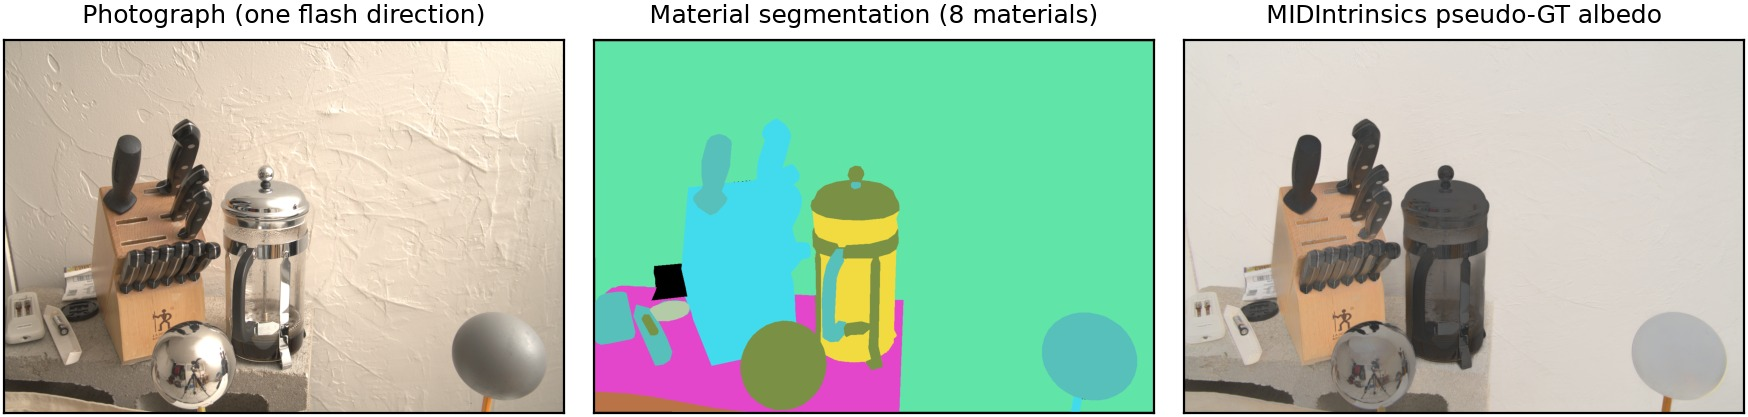
\includegraphics[width=\textwidth]{images/report/mid_materials.jpg}
  \caption[What the MID scores are computed on.]{%
    What the MID scores are computed on. Each test scene comes with a segmentation into
    material regions (middle). $C_{\text{mat}}$ and $\text{Cast}_{\text{rel}}$ compare the mean
    predicted albedo of each region across the flash directions, and
    $\text{Chroma}_{\text{err}}$ compares it with the MIDIntrinsics pseudo-ground truth (right).
  }
  \label{fig:mid_materials}
\end{figure}

The first score asks whether the material's \emph{luminance} holds still.
Writing $\mu_{m,k}$ for the mean luminance of the predicted albedo over material $m$
in frame $k$, we take the coefficient of variation across frames and average it over
materials,
\begin{equation}
  C_{\text{mat}} \;=\;
  \frac{1}{|M|} \sum_{m \in M}
  \frac{\operatorname{std}_k\bigl(\mu_{m,k}\bigr)}
       {\operatorname{mean}_k\bigl(\mu_{m,k}\bigr)} .
  \label{eq:cmat}
\end{equation}
Dividing by the mean makes the score scale-free, which matters because albedo is only
defined up to a global scale.

\begin{figure}[t!]
  \centering
  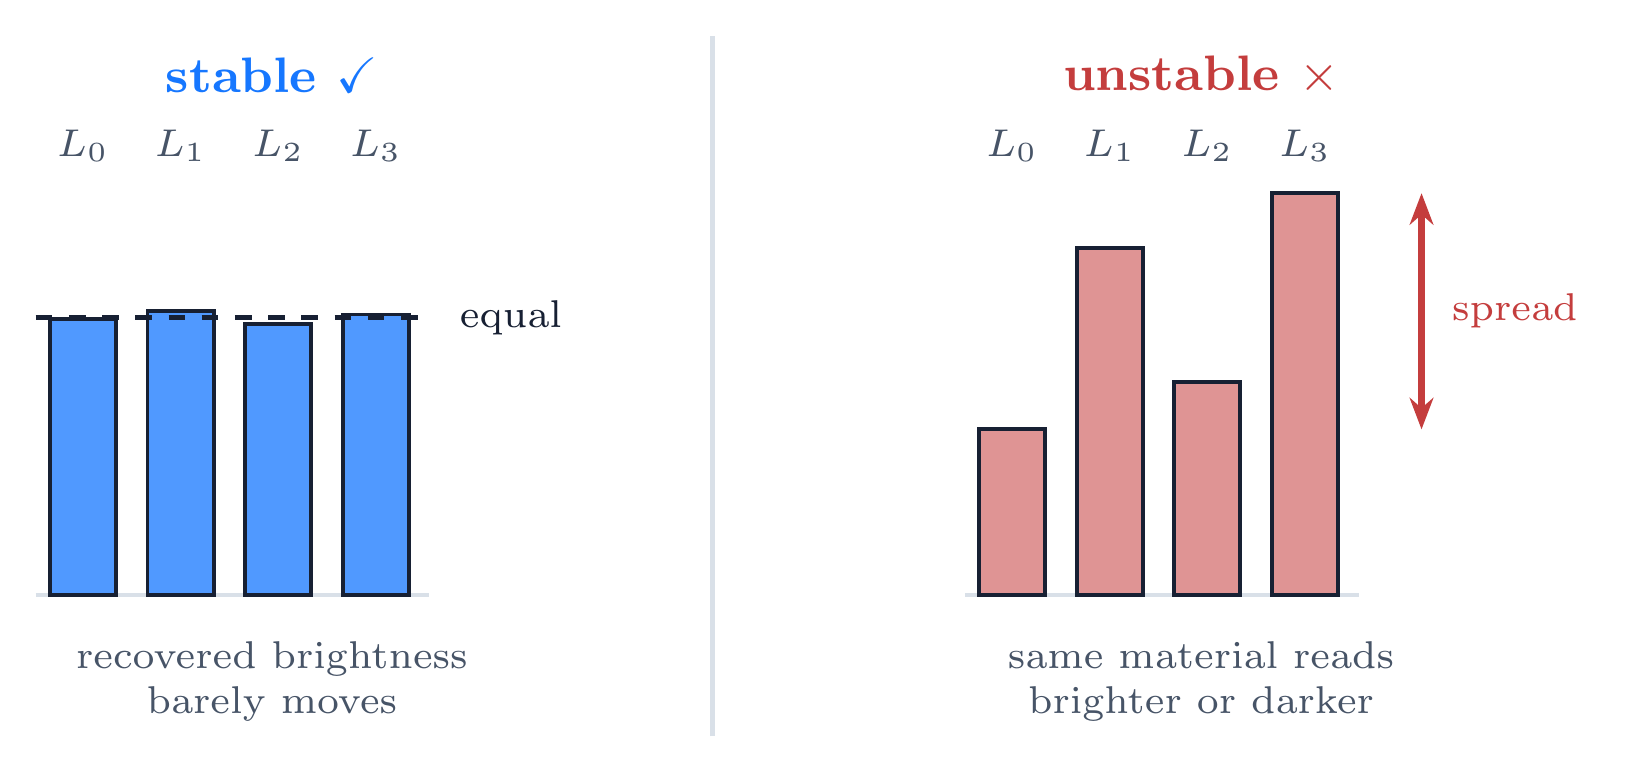
\includegraphics[width=0.72\textwidth]{images/losses/metric_card_cmat.png}
  \caption[$C_{\text{mat}}$: four illuminants, one material.]{%
    $C_{\text{mat}}$ is the coefficient of variation of one material's mean
    luminance across the scene's illuminant conditions. A stable prediction gives
    four nearly equal bars; a prediction whose brightness tracks the lamp gives
    four bars with visible spread, which is exactly the quantity the standard
    deviation in \eqnref{eq:cmat} measures.
  }
  \label{fig:metric_card_cmat}
\end{figure}

The second score asks whether the material's \emph{colour} holds still, which is the
axis a coloured lamp actually attacks. We reduce each material in each frame to its
two chromaticity ratios $r_{m,k} = \bar{A}^{R}_{m,k} / \bar{A}^{G}_{m,k}$ and
$b_{m,k} = \bar{A}^{B}_{m,k} / \bar{A}^{G}_{m,k}$. Normalising by the green channel
removes brightness and leaves hue, so a model that lets a warm lamp tint its albedo
will show drift in $r_{m,k}$ and $b_{m,k}$ even if its luminance is stable.

\paragraph{Reported metrics}
Pooling these ratios over every material and frame is not a stability score: the pooled
spread also contains the chroma differences \emph{between} materials, so a model that pulls
all materials toward one hue lowers it without being more stable (in the ablation of
\secref{sec:ablation} it ranks the visibly desaturated configuration best). We therefore
keep only the drift \emph{within} each material. Write the
per-material drift and the between-material chroma spread of a prediction $A$ as
\begin{equation}
  \delta_m \;=\; \sqrt{\operatorname{Var}_k(r_{m,k}) + \operatorname{Var}_k(b_{m,k})} ,
  \qquad
  S(A) \;=\; \sqrt{\operatorname{Var}_m\bigl(\bar{r}_m\bigr) + \operatorname{Var}_m\bigl(\bar{b}_m\bigr)} ,
  \label{eq:castterms}
\end{equation}
with $\bar{r}_m = \mathbb{E}_k[r_{m,k}]$ and $\bar{b}_m = \mathbb{E}_k[b_{m,k}]$. The
constancy score is the mean drift measured against the chroma scale the model actually
uses,
\begin{equation}
  \text{Cast}_{\text{rel}} \;=\;
  \frac{\tfrac{1}{|M|}\sum_{m \in M} \delta_m}{S(A)} ,
  \label{eq:castrel}
\end{equation}
a coefficient of variation in chroma. The normalisation is necessary because $\delta_m$
is an absolute quantity: a model that carries twice as much albedo chroma has twice as
much room to drift in absolute units, so comparing raw $\delta_m$ across models with
different colourfulness penalises the more colourful one for being colourful.
$\text{Cast}_{\text{rel}}$ instead asks the question that matters perceptually: whether
two materials remain distinguishable when the lighting changes. Being a ratio, it has one
blind spot: a change that lowers the drift and the model's own chroma by the same
fraction leaves it unchanged.

\begin{figure}[t!]
  \centering
  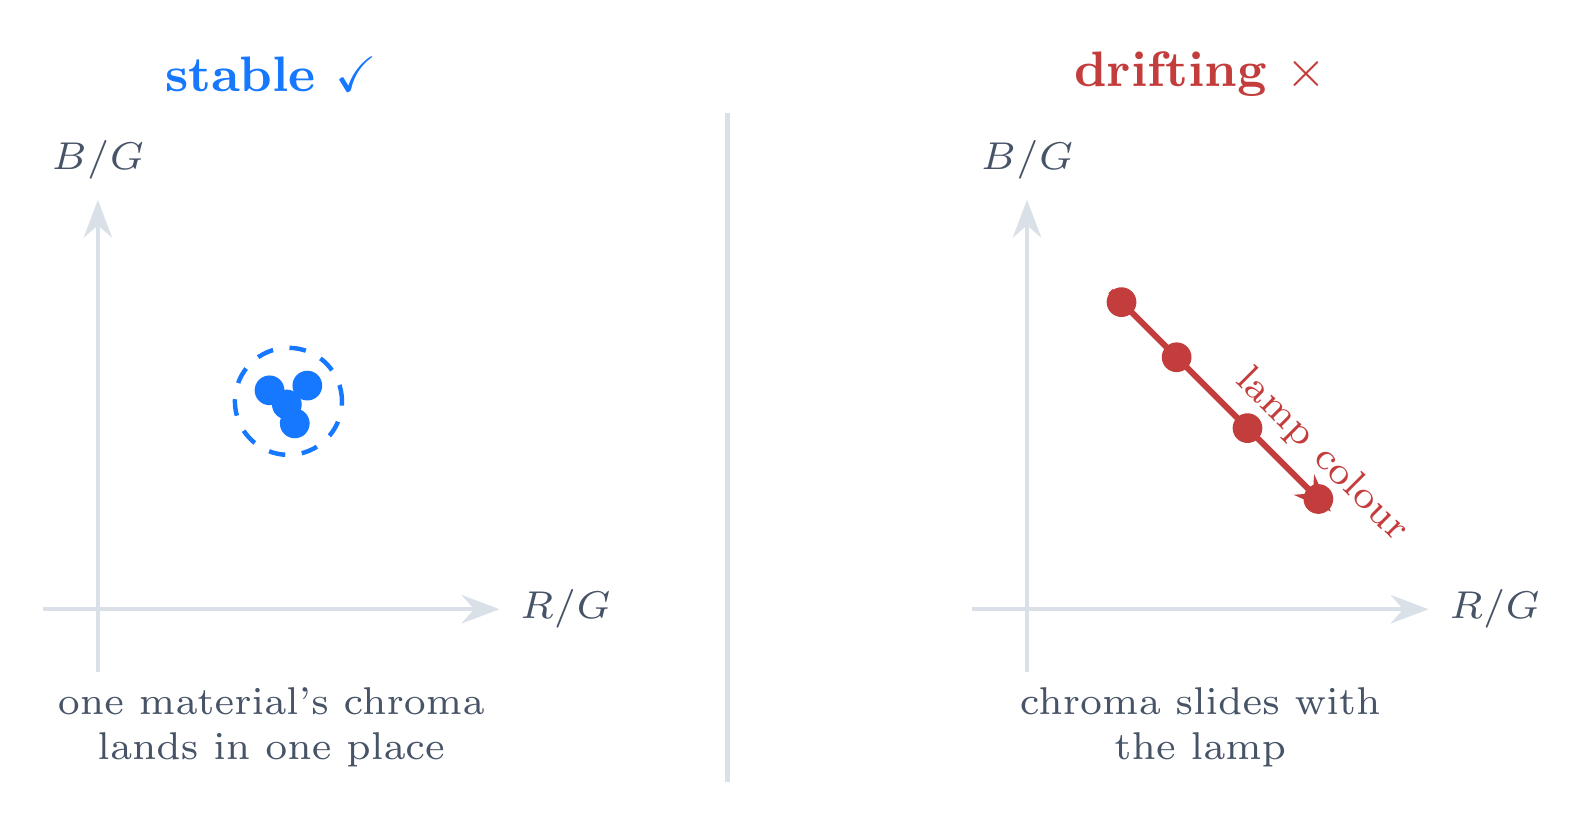
\includegraphics[width=0.72\textwidth]{images/losses/metric_card_castrel.png}
  \caption[$\text{Cast}_{\text{rel}}$: one material's chroma across illuminants.]{%
    Plotting one material's per-illuminant chromaticity $(r_{m,k}, b_{m,k})$ as a
    scatter makes the two failure modes visually distinct: a stable material clusters
    tightly, while a material whose colour tracks the lamp strings out along the
    illuminant-colour direction. $\delta_m$ (\eqnref{eq:castterms}) is the radius of
    that cluster.
  }
  \label{fig:metric_card_castrel}
\end{figure}

\paragraph{Accuracy beside stability}
Stability alone can never be reported on its own, because a constant predictor attains
it: a model that emits flat grey albedo is \emph{perfectly} stable and scores zero on
every drift measure. Every stability number in this chapter is therefore read next to
an accuracy number. The external accuracy measure is MAW (\secref{sec:maw_results}):
CIEDE2000 error against physically measured albedo, comparable with published tables.
It is not sufficient here on its own, for two reasons. It scores different photographs,
one illumination each, so it cannot tell whether the very frames on which stability was
measured were washed out; and it does not reliably register desaturation. CRefNet, whose albedo
is visibly pale on MID, scores a MAW $\Delta E$ of
$3.970$, better than our model's $4.155$, although MAW does separate our own
desaturated ablation row from its colour-preserving counterpart ($4.631$ against $4.155$).
We therefore add an in-domain accuracy measure on the same MID frames, the mean
per-material chromaticity error against the pseudo-ground truth,
\begin{equation}
  \text{Chroma}_{\text{err}} \;=\;
  \frac{1}{|M|}\sum_{m\in M}\bigl\lVert (\bar r_m,\bar b_m) - (\bar r^{*}_m,\bar b^{*}_m)\bigr\rVert,
  \label{eq:chromaerr}
\end{equation}
where $(\bar r^{*}_m,\bar b^{*}_m)$ is the pseudo-GT chromaticity of material $m$; lower
is better. This is an ordinary accuracy measure, restricted to chromaticity, not a new
metric. Its limitation is the reference itself: the pseudo-ground truth is derived from
MID's capture stack, and both our model and CD-IID train on MIDIntrinsics.

\begin{figure}[t!]
  \centering
  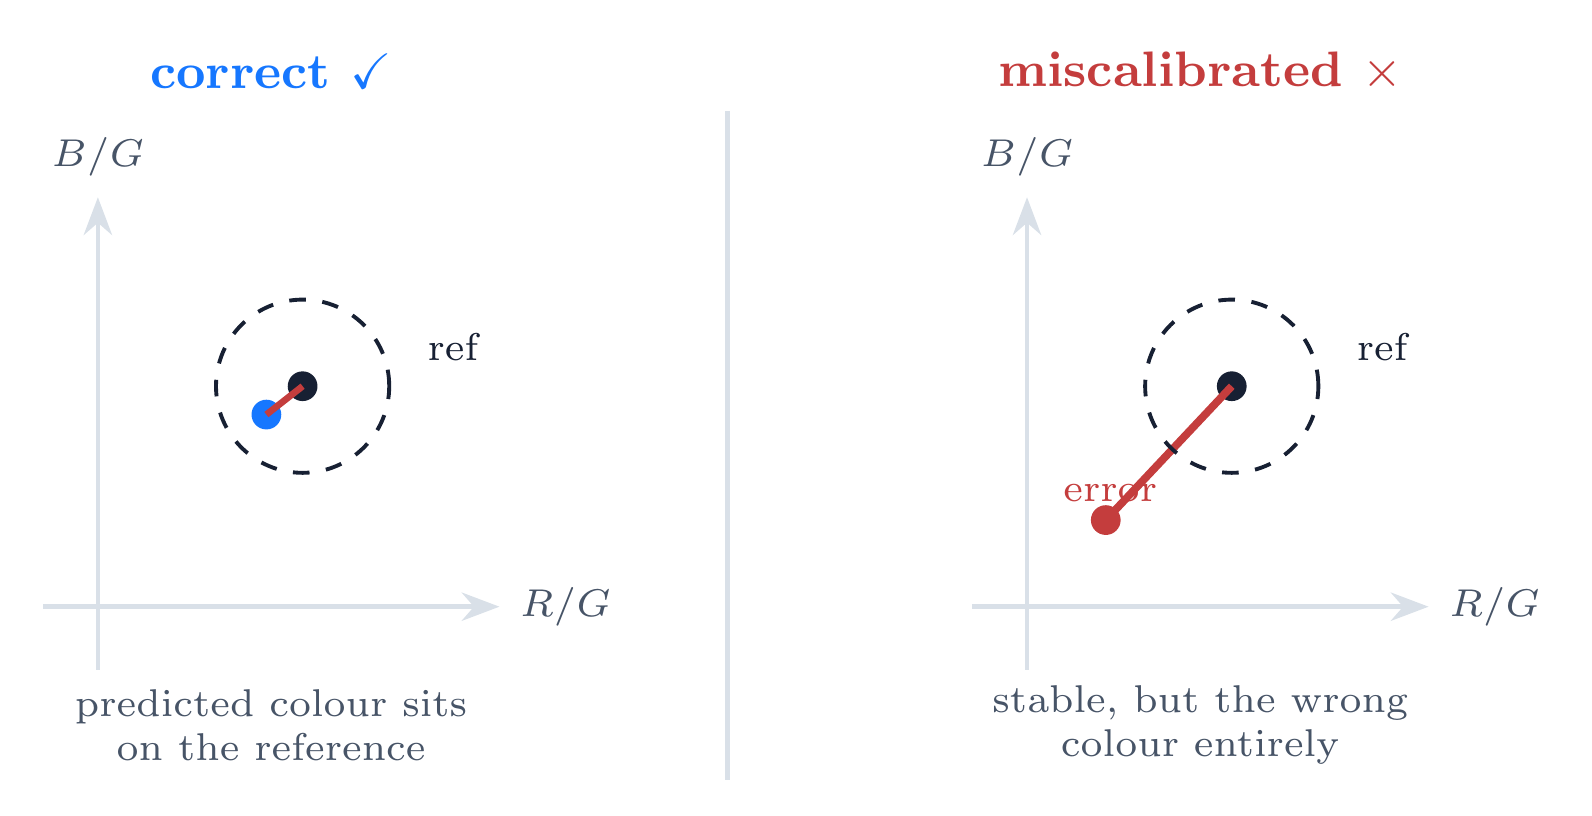
\includegraphics[width=0.72\textwidth]{images/losses/metric_card_chromaerr.png}
  \caption[$\text{Chroma}_{\text{err}}$: stable is not the same as correct.]{%
    $\text{Cast}_{\text{rel}}$ alone cannot see this failure: a prediction can be
    perfectly clustered (stable) yet sit on entirely the wrong point in chroma space.
    $\text{Chroma}_{\text{err}}$ is the distance from that cluster to the pseudo-GT
    reference, so it is zero only when the stable colour is also the right one.
  }
  \label{fig:metric_card_chromaerr}
\end{figure}

$C_{\text{mat}}$ and $\text{Cast}_{\text{rel}}$ are lower-is-better and both vanish for
a perfectly illuminant-invariant prediction. They are reported separately, rather than
combined, because they can move in opposite directions: $C_{\text{mat}}$ is a luminance
score and $\text{Cast}_{\text{rel}}$ a hue score, and a configuration may stabilise one
while disturbing the other.

For ARAP, which has no material segmentation, the stability score is computed per pixel.
For a group of $N$ renderings of one scene, $C_{\text{arap}}$ takes the coefficient of
variation of the predicted albedo luminance across the renderings at every valid pixel, and
averages it over the valid pixels $\Omega_g$ of the group and then over the groups $G$,
\begin{equation}
  C_{\text{arap}} \;=\;
  \frac{1}{|G|} \sum_{g \in G} \frac{1}{|\Omega_g|} \sum_{p \in \Omega_g}
  \frac{\operatorname{std}_k L\bigl(\mathbf{A}_k(p)\bigr)}
       {\operatorname{mean}_k L\bigl(\mathbf{A}_k(p)\bigr)} ,
  \label{eq:carap}
\end{equation}
where $L$ is the Rec.~709 luminance and a pixel is valid when its ground-truth albedo
luminance exceeds $0.004$. Like
$C_{\text{mat}}$, it is a luminance score. The accuracy scores of MAW and IIW are defined with
their benchmarks (\secref{sec:maw_results} and \secref{sec:iiw_results}).

\section{MID: Stability Across Flash Directions}
\label{sec:mid_results}

The purpose of this section is to measure, directly, whether the predicted albedo stays
the same when only the light changes. MID \mycite{midintrinsics} photographs each real room
25 times and moves only the flash, so it isolates this variable. Its albedo is a
pseudo-ground truth rather than a measurement, so MID is mainly a stability test; accuracy
is checked against measured albedo on MAW (\secref{sec:maw_results}). We use the held-out
30-scene test split and the scores of \secref{sec:metrics}.

MID is in-domain for two methods. We train on the official MID training split, and CD-IID
\mycite{careaga24cdiid} also trains on MID but does not state which split it used, so we
cannot verify which test scenes it saw. The table therefore compares locally evaluated models
under one pipeline and makes no zero-shot claim.

\begin{table}[t!]
  \caption[MID stability and chroma accuracy.]{%
    Stability and in-domain accuracy on the held-out MIDIntrinsics test split
    \mycite{midintrinsics}, 30 scenes; brackets are $95\%$ percentile-bootstrap intervals
    over scenes ($20{,}000$ resamples). $C_{\text{mat}}$ (\eqnref{eq:cmat}) is luminance stability and
    $\text{Cast}_{\text{rel}}$ (\eqnref{eq:castrel}) is scale-normalised hue stability;
    $\text{Chroma}_{\text{err}}$ (\eqnref{eq:chromaerr}) is the per-material chromaticity
    error against the pseudo-ground truth. Lower is better for all three. Red, orange,
    and yellow mark first, second, and third numerical rank; the bootstrap intervals and
    the paired tests of \tabref{tab:mid_paired}, not the colour fill, decide whether a
    difference is supported. These are our own measures, so no published method
    reports comparable values; every row is evaluated locally under one pipeline.
  }
  \label{tab:mid}
  \centering
  \small
  \resizebox{\textwidth}{!}{%
  \begin{tabular}{@{}lccc@{}}
    \toprule
    Model & $C_{\text{mat}}$ $\downarrow$ & $\text{Chroma}_{\text{err}}$ $\downarrow$
          & $\text{Cast}_{\text{rel}}$ $\downarrow$ \\
    \midrule
    Ours                                       & \rankthree{0.157\,{\scriptsize[.142,.175]}} & \ranktwo{0.129\,{\scriptsize[.110,.150]}} & 0.425\,{\scriptsize[.360,.492]} \\
    CD-IID \mycite{careaga24cdiid}             & 0.190\,{\scriptsize[.172,.210]} & \rankone{0.090\,{\scriptsize[.073,.110]}} & \rankone{0.306\,{\scriptsize[.262,.355]}} \\
    RGB$\rightarrow$X \mycite{zeng24rgbx}      & \rankone{0.128\,{\scriptsize[.115,.141]}} & 0.203\,{\scriptsize[.170,.239]} & \ranktwo{0.338\,{\scriptsize[.273,.409]}} \\
    Marigold-App \mycite{marigoldiid24}        & 0.193\,{\scriptsize[.173,.214]} & 0.195\,{\scriptsize[.152,.245]} & \rankthree{0.355\,{\scriptsize[.309,.406]}} \\
    Marigold-Light \mycite{marigoldiid24}      & 0.546\,{\scriptsize[.463,.645]} & 0.154\,{\scriptsize[.125,.186]} & 0.392\,{\scriptsize[.333,.460]} \\
    CRefNet \mycite{luo23crefnet}              & \ranktwo{0.151\,{\scriptsize[.138,.164]}} & 0.201\,{\scriptsize[.165,.241]} & \rankthree{0.355\,{\scriptsize[.308,.405]}} \\
    Ordinal Shading \mycite{careaga23ordinal}  & 0.252\,{\scriptsize[.229,.280]} & \rankthree{0.148\,{\scriptsize[.130,.166]}} & 0.549\,{\scriptsize[.463,.638]} \\
    \bottomrule
  \end{tabular}}
\end{table}

The first thing we can see from \tabref{tab:mid} is that our model does not lead any single
column. We start with the two columns where it trails, using the paired bootstrap of
\tabref{tab:mid_paired} to decide which differences are significant.

First, our model does \emph{not} lead hue stability. Every external method except Ordinal Shading
has a lower $\text{Cast}_{\text{rel}}$ than our $0.425$, and the paired difference is
significant for four of the five. CD-IID leads the column at $0.306$.

Second, it does not lead chroma accuracy either. Its $\text{Chroma}_{\text{err}}$ of $0.129$ is second
to CD-IID's $0.090$, and that gap is significant ($+0.039\,[+0.022, +0.057]$). CD-IID reaches
better accuracy \emph{and} better hue stability while keeping its colour. In other words,
low hue drift can be reached without desaturating the albedo.

On luminance, however, our model is significantly more stable than CD-IID, both Marigold
variants and Ordinal Shading. It is level with CRefNet, with a paired difference of
$+0.007\,[-0.004, +0.019]$, and significantly less stable than RGB$\rightarrow$X
($+0.030\,[+0.014, +0.047]$). This comparison across methods mixes
architectures, training data and model size, so it does not isolate the training strategy;
the matched ablation of \secref{sec:ablation} does, and the claim of this thesis rests on it.

\begin{table}[t!]
  \caption[Paired comparisons against each external baseline.]{%
    Paired differences on the held-out MID split, our model minus each external
    baseline, scene by scene. All three metrics are lower-is-better, so a negative
    entry means our model wins. Brackets are $95\%$ percentile-bootstrap intervals
    over the $30$ scenes ($20{,}000$ resamples); \textbf{bold} marks an interval
    clear of zero. Because every method is scored on the same scenes, the difference
    can be taken per scene, which cancels scene difficulty. Reproduce with
    \texttt{tests/eval/paired\_bootstrap\_mid.py}.
  }
  \label{tab:mid_paired}
  \centering
  \small
  \resizebox{\textwidth}{!}{%
  \begin{tabular}{@{}lccc@{}}
    \toprule
    Ours $-$ & $C_{\text{mat}}$ & $\text{Chroma}_{\text{err}}$ & $\text{Cast}_{\text{rel}}$ \\
    \midrule
    CD-IID \mycite{careaga24cdiid}               & \textbf{-0.032\,{\scriptsize[-0.045,-0.019]}} & \textbf{+0.039\,{\scriptsize[+0.022,+0.057]}} & \textbf{+0.119\,{\scriptsize[+0.085,+0.156]}} \\
    RGB$\rightarrow$X \mycite{zeng24rgbx}        & \textbf{+0.030\,{\scriptsize[+0.014,+0.047]}} & \textbf{-0.074\,{\scriptsize[-0.104,-0.045]}} & \textbf{+0.087\,{\scriptsize[+0.024,+0.149]}} \\
    CRefNet \mycite{luo23crefnet}                & +0.007\,{\scriptsize[-0.004,+0.019]} & \textbf{-0.072\,{\scriptsize[-0.102,-0.044]}} & \textbf{+0.070\,{\scriptsize[+0.030,+0.117]}} \\
    Marigold-App \mycite{marigoldiid24}          & \textbf{-0.035\,{\scriptsize[-0.055,-0.016]}} & \textbf{-0.067\,{\scriptsize[-0.103,-0.032]}} & \textbf{+0.070\,{\scriptsize[+0.030,+0.111]}} \\
    Marigold-Light \mycite{marigoldiid24}        & \textbf{-0.388\,{\scriptsize[-0.484,-0.308]}} & -0.025\,{\scriptsize[-0.055,+0.004]} & +0.033\,{\scriptsize[-0.020,+0.085]} \\
    Ordinal Shading \mycite{careaga23ordinal}    & \textbf{-0.095\,{\scriptsize[-0.117,-0.075]}} & \textbf{-0.019\,{\scriptsize[-0.035,-0.003]}} & \textbf{-0.124\,{\scriptsize[-0.160,-0.094]}} \\
    \bottomrule
  \end{tabular}}
\end{table}

Reading stability and accuracy together separates three behaviours among the seven rows.
CRefNet is \emph{stable but pale}: a low $\text{Cast}_{\text{rel}}$ next to a high
$\text{Chroma}_{\text{err}}$ ($0.201$) and a visibly washed-out albedo (\figref{fig:comp_grid}).
RGB$\rightarrow$X is \emph{colourful but miscalibrated}: it keeps strong colours but on the
wrong hues, with the worst $\text{Chroma}_{\text{err}}$ in the table ($0.203$). CD-IID is good on both.

% MID hue stability vs chroma error (values from documents/results/mid_per_scene.json).
% x = Cast_rel (lower is better); y = Chroma_err against MID pseudo-GT (lower is better).
\begin{figure}[t!]
  \centering
  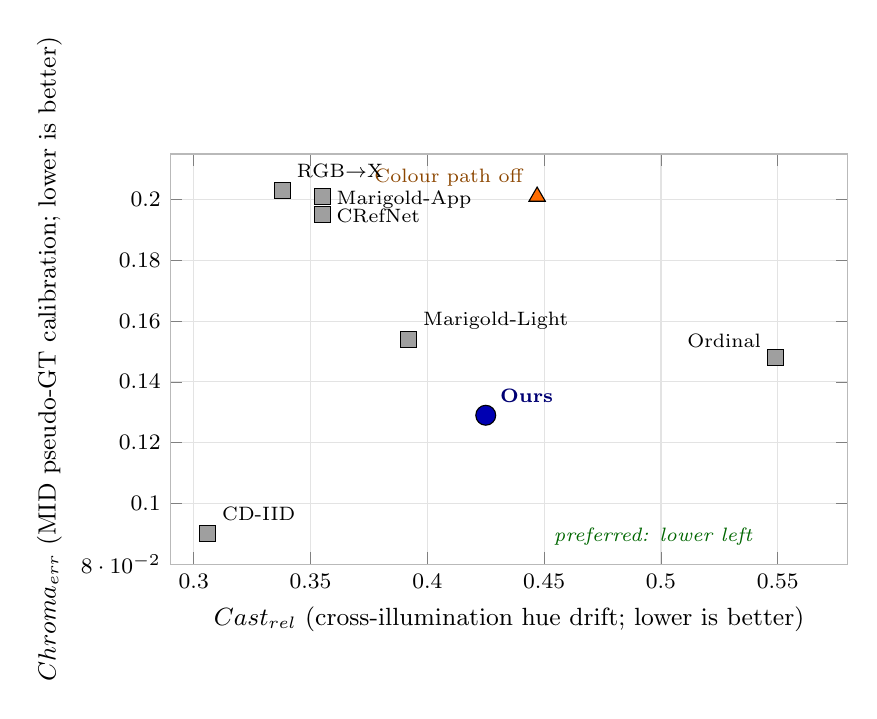
\begin{tikzpicture}
    \begin{axis}[
        width=0.84\textwidth, height=0.56\textwidth,
        xlabel={$\text{Cast}_{\text{rel}}$ (cross-illumination hue drift; lower is better)},
        ylabel={$\text{Chroma}_{\text{err}}$ (MID pseudo-GT calibration; lower is better)},
        xlabel style={font=\small}, ylabel style={font=\small},
        tick label style={font=\footnotesize},
        xmin=0.29, xmax=0.58,
        ymin=0.08, ymax=0.215,
        grid=major,
        grid style={gray!22},
        axis line style={gray!55},
        clip=false,
      ]
      \node[anchor=south west, font=\scriptsize\itshape, text=green!40!black]
        at (axis cs:0.45,0.083) {preferred: lower left};

      \addplot[only marks, mark=*, mark size=3.6pt, draw=black, fill=blue!70!black]
        coordinates {(0.425,0.129)};
      \node[anchor=south west, font=\scriptsize\bfseries, blue!45!black]
        at (axis cs:0.427,0.130) {Ours};

      \addplot[only marks, mark=triangle*, mark size=3.4pt, draw=black, fill=orange!85!red]
        coordinates {(0.447,0.201)};
      \node[anchor=south east, font=\scriptsize, orange!55!black]
        at (axis cs:0.445,0.201) {Colour path off};

      \addplot[only marks, mark=square*, mark size=2.9pt, draw=black, fill=gray!75]
        coordinates {(0.355,0.195) (0.392,0.154) (0.355,0.201) (0.549,0.148) (0.306,0.090) (0.338,0.203)};
      \node[anchor=south west, font=\scriptsize] at (axis cs:0.357,0.194) {Marigold-App};
      \node[anchor=south west, font=\scriptsize] at (axis cs:0.394,0.154) {Marigold-Light};
      \node[anchor=north west, font=\scriptsize] at (axis cs:0.357,0.200) {CRefNet};
      \node[anchor=south east, font=\scriptsize] at (axis cs:0.547,0.148) {Ordinal};
      \node[anchor=south west, font=\scriptsize] at (axis cs:0.308,0.091) {CD-IID};
      \node[anchor=south west, font=\scriptsize] at (axis cs:0.340,0.204) {RGB$\rightarrow$X};
    \end{axis}
  \end{tikzpicture}
  \caption[MID hue stability versus pseudo-GT chroma error.]{%
    Hue drift across flash directions against chroma error to the pseudo-GT on the
    30-scene MID test split; lower is better on both axes. CD-IID is best on both.
    Marigold-App and CRefNet drift less than our model but with substantially higher
    chroma error, and so does our own configuration without the colour path.
  }
  \label{fig:tradeoff}
\end{figure}


\figref{fig:tradeoff} plots hue stability against pseudo-GT chroma error for the roster.
Lower is better on both axes. CRefNet and Marigold-App drift less than our model but with
substantially higher chroma error, and the colour-path-off ablation sits in the same
high-error region; CD-IID is best on both axes.

\figref{fig:cmat_vs_chroma} shows the same roster on the score the claim rests on.
Lower is better on both axes. Our model sits in the lower-left group with CRefNet, RGB$\rightarrow$X
and CD-IID on luminance stability, and of those, only CD-IID is more accurate in chroma.

\begin{figure}[t!]
  \centering
  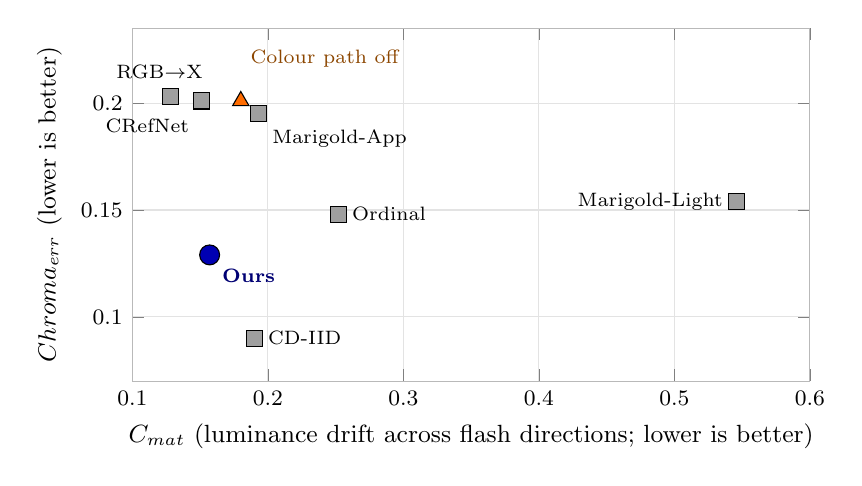
\begin{tikzpicture}
    \begin{axis}[
        width=0.84\textwidth, height=0.5\textwidth,
        xlabel={$C_{\text{mat}}$ (luminance drift across flash directions; lower is better)},
        ylabel={$\text{Chroma}_{\text{err}}$ (lower is better)},
        xlabel style={font=\small}, ylabel style={font=\small},
        tick label style={font=\footnotesize},
        xmin=0.10, xmax=0.60, ymin=0.07, ymax=0.235,
        grid=major, grid style={gray!22}, axis line style={gray!55}, clip=false]
      \addplot[only marks, mark=*, mark size=3.6pt, draw=black, fill=blue!70!black] coordinates {(0.157,0.129)};
      \node[anchor=north west, font=\scriptsize\bfseries, blue!45!black] at (axis cs:0.159,0.127) {Ours};
      \addplot[only marks, mark=triangle*, mark size=3.4pt, draw=black, fill=orange!85!red] coordinates {(0.180,0.201)};
      \node[anchor=south west, font=\scriptsize, orange!55!black] at (axis cs:0.180,0.212) {Colour path off};
      \addplot[only marks, mark=square*, mark size=2.9pt, draw=black, fill=gray!75]
        coordinates {(0.190,0.090) (0.128,0.203) (0.151,0.201) (0.193,0.195) (0.546,0.154) (0.252,0.148)};
      \node[anchor=west, font=\scriptsize] at (axis cs:0.193,0.090) {CD-IID};
      \node[anchor=south, font=\scriptsize] at (axis cs:0.120,0.207) {RGB$\rightarrow$X};
      \node[anchor=north east, font=\scriptsize] at (axis cs:0.149,0.197) {CRefNet};
      \node[anchor=north west, font=\scriptsize] at (axis cs:0.196,0.192) {Marigold-App};
      \node[anchor=east, font=\scriptsize] at (axis cs:0.543,0.154) {Marigold-Light};
      \node[anchor=west, font=\scriptsize] at (axis cs:0.255,0.148) {Ordinal};
    \end{axis}
  \end{tikzpicture}
  \caption[MID luminance stability versus chroma error.]{%
    Luminance stability against chroma error on the 30-scene MID test split (values of
    \tabref{tab:mid}); lower is better on both axes. ``Colour path off'' is Row~2 of the
    ablation (\secref{sec:ablation}).
  }
  \label{fig:cmat_vs_chroma}
\end{figure}

\figref{fig:intro_constancy} in \chapref{ch:intro} shows a qualitative example: each
column is a different flash direction for the same scene, and the variation map shows
where the predicted luminance changes with the light.
\figref{fig:mid_grid} puts all seven methods side by side on one held-out scene. Reading
down each column shows how much a method's albedo changes with the flash direction, and
comparing each column with the pseudo-ground truth shows how accurate it is. The three
behaviours described above are visible here: CRefNet stays steady but pale, RGB$\rightarrow$X
keeps strong colours but drops the colour of the blue jacket at light 18, and Marigold-Light
changes the most between rows. Our albedo changes little between rows but is paler than the
pseudo-ground truth.

\begin{figure}[t!]
  \centering
  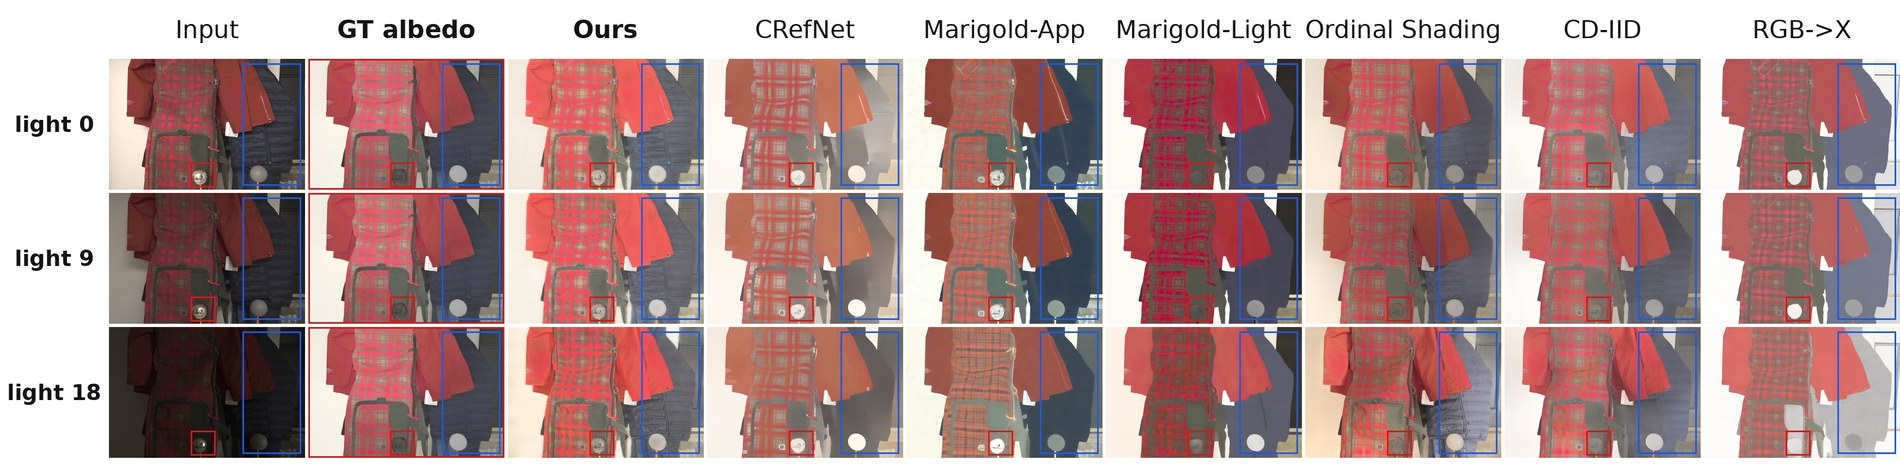
\includegraphics[width=\textwidth]{images/readme/ciai-qualitative.jpg}
  \caption[MID albedo of all seven methods under three flash directions.]{%
    One held-out MID scene under three flash directions (rows) for all seven methods
    (columns), next to the input and the pseudo-ground-truth albedo. The red and blue boxes
    mark the same two regions in every panel, a small metal sphere and the blue jacket, so
    any change down a column comes from the model. With per-scene $C_{\text{mat}}$ from the
    model of \tabref{tab:mid}, RGB$\rightarrow$X is about as steady in brightness as ours on
    this scene ($0.18$ against $0.19$) but loses the jacket's colour at light 18; CRefNet
    ($0.26$) and Marigold-Light ($0.41$) change more. One scene cannot rank the methods;
    \tabref{tab:mid} does.
  }
  \label{fig:mid_grid}
\end{figure}




\section{Ablation Study}
\label{sec:ablation}

The benchmark sections placed our model against external methods, which differ from it in
architecture, data and size at once. The purpose of this section is to isolate what CIAI
itself contributes, with a $2\times2$ ablation inside our own architecture.

The two axes of the ablation are whether the cross-illumination losses
($\mathcal{L}_{\text{inv}}$, $\mathcal{L}_{\text{expl}}$) are active, and whether the colour
path (the RGB skip into the albedo head and the chroma loss on albedo,
\secref{sec:architecture}) is active. All four configurations start from the same 19k
checkpoint and follow the same data schedule to 40k iterations (\secref{sec:schedule}).
\tabref{tab:ablation} reports the results in three parts: stability on raw inputs (Part~1),
accuracy under the standard protocols (Part~2a), and dense accuracy on raw ARAP inputs
(Part~2b).

Only two comparisons are causal tests of CIAI: Row~1$\rightarrow$Row~2 adds the
cross-illumination losses with the colour path off, and Row~3$\rightarrow$Row~4 adds them
with the colour path on. The comparison across the colour-path axis is descriptive only.
Switching the colour path changes the shape of the albedo head, so the optimiser state of the
19k checkpoint could not be restored on that side, and Adam restarted with empty moment
estimates. This changed the effective learning rate by about $1.85\times$, so we do not
attribute cross-axis differences to the colour path alone. All rows are single training runs,
so small differences should not be read as effects.

\begin{table}[p]
  \caption[CIAI ablation across constancy and accuracy.]{%
    The $2\times2$ CIAI ablation. All rows start from the same 19k checkpoint and train to
    40k; Row~1$\rightarrow$Row~2 and Row~3$\rightarrow$Row~4 are the matched comparisons.
    Part~1: stability on raw inputs, with ARAP on the $16$/$11$ colour-varying groups of
    \tabref{tab:arap_constancy}. Part~2a: MAW accuracy, ARAP accuracy on white-balanced
    inputs, and IIW. Part~2b: ARAP accuracy on raw inputs. All ARAP columns use the
    evaluation mask of \secref{sec:arap_results}.
    Lower is better everywhere except ARAP SSIM. Best per column is \textbf{bold}.
    \figref{fig:ablation} shows the corresponding albedo and variation maps.
  }
  \label{tab:ablation}
  \centering
  \textbf{\small Part 1: Raw-input constancy (self-consistency across illuminants)}\\[2pt]
  \resizebox{\textwidth}{!}{%
  \begin{tabular}{@{}lllccccc@{}}
    \toprule
    & & & \multicolumn{3}{c}{MID (30 scenes)} & ARAP all & ARAP indoor \\
    \cmidrule(lr){4-6}\cmidrule(lr){7-7}\cmidrule(l){8-8}
    Row & Cross-illumination & Colour path
        & $C_{\text{mat}}$ $\downarrow$ & $\text{Cast}_{\text{rel}}$ $\downarrow$
        & $\text{Chroma}_{\text{err}}$ $\downarrow$
        & $C_{\text{arap}}$ $\downarrow$ & $C_{\text{arap}}$ $\downarrow$ \\
    \midrule
    1 & off & off & 0.250 & 0.477 & 0.186 & 0.164 & 0.122 \\
    2 & on  & off & 0.180 & 0.447 & 0.201 & \textbf{0.145} & \textbf{0.108} \\
    3 & off & on  & 0.259 & 0.444 & \textbf{0.124} & 0.155 & 0.117 \\
    4 & on  & on  & \textbf{0.157} & \textbf{0.425} & 0.129 & 0.154 & 0.119 \\
    \bottomrule
  \end{tabular}}\\[3pt]
  {\footnotesize ARAP has no material segmentation, so it contributes the per-pixel
  luminance score $C_{\text{arap}}$ (\eqnref{eq:carap}) but no hue or chroma score.}\\[4pt]
  \textbf{\small Part 2a: Standard-protocol accuracy and structure (against ground truth)}\\[2pt]
  \resizebox{\textwidth}{!}{%
  \begin{tabular}{@{}lllcccccc@{}}
    \toprule
    & & & \multicolumn{2}{c}{MAW} & \multicolumn{3}{c}{ARAP (GT-achromatized)} & \multicolumn{1}{c}{IIW} \\
    \cmidrule(lr){4-5}\cmidrule(lr){6-8}\cmidrule(l){9-9}
    Row & Cross-illumination & Colour path & $\Delta E$ $\downarrow$ & Int.$\times$100 $\downarrow$ & LMSE$^\dagger$ $\downarrow$ & mn-RMSE$^\dagger$ $\downarrow$ & SSIM$^\dagger$ $\uparrow$ & WHDR $\downarrow$ \\
    \midrule
    1 & off & off & 4.434 & 0.409 & 0.0307 & 0.2378 & 0.602 & 0.334 \\
    2 & on  & off & 4.631 & 0.474 & 0.0320 & 0.2313 & 0.589 & \textbf{0.283} \\
    3 & off & on  & \textbf{4.115} & \textbf{0.395} & 0.0283 & 0.2348 & \textbf{0.617} & 0.327 \\
    4 & on  & on  & 4.155 & 0.504 & \textbf{0.0279} & \textbf{0.2259} & 0.611 & 0.286 \\
    \bottomrule
  \end{tabular}}\\[5pt]
  \textbf{\small Part 2b: Raw-input ARAP albedo accuracy (against ground truth)}\\[2pt]
  \resizebox{\textwidth}{!}{%
  \begin{tabular}{@{}lllcccc@{}}
    \toprule
    & & & \multicolumn{2}{c}{All ARAP (raw input)}
        & \multicolumn{2}{c}{Indoor ARAP (raw input)} \\
    \cmidrule(lr){4-5}\cmidrule(l){6-7}
    Row & Cross-illumination & Colour path
        & LMSE $^\ddagger$ $\downarrow$ & mn-RMSE $^\ddagger$ $\downarrow$
        & LMSE $^\ddagger$ $\downarrow$ & mn-RMSE $^\ddagger$ $\downarrow$ \\
    \midrule
    1 & off & off & 0.0463 & 0.341 & 0.0441 & 0.323 \\
    2 & on  & off & 0.0397 & \textbf{0.292} & \textbf{0.0370} & \textbf{0.275} \\
    3 & off & on  & 0.0426 & 0.319 & 0.0400 & 0.301 \\
    4 & on  & on  & \textbf{0.0396} & 0.293 & 0.0382 & 0.276 \\
    \bottomrule
  \end{tabular}}\\[3pt]
  {\footnotesize $\dagger$ GT-achromatized ARAP accuracy guard (136 of 157 images): an internal
  within-study comparison, not a reproduced literature table. IIW WHDR is ancillary and is
  not a selection criterion. $\ddagger$ Raw-input ARAP accuracy is a local multi-illuminant
  stress test and is not compared with published white-balanced results.}
\end{table}

\paragraph{Effect of cross-illumination losses within each architecture}
\figref{fig:ablation_deltas} summarises the two matched comparisons as relative changes.

\begin{figure}[t!]
  \centering
  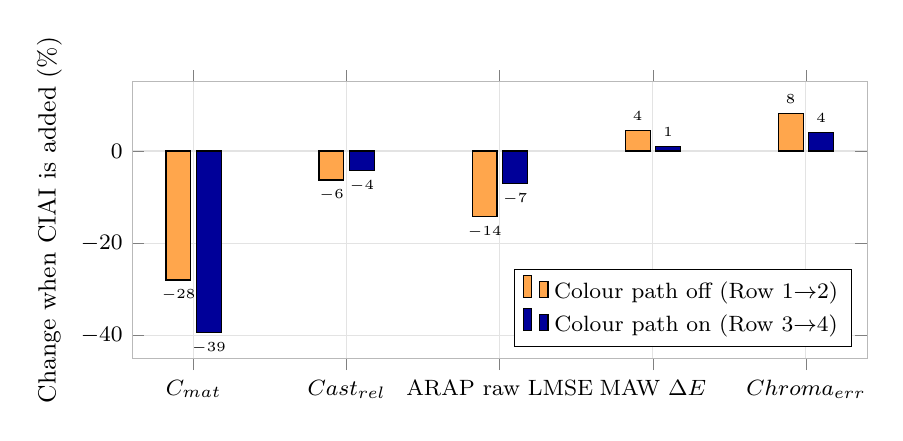
\begin{tikzpicture}
    \begin{axis}[
        ybar, bar width=9pt, width=0.9\textwidth, height=0.42\textwidth,
        ylabel={Change when CIAI is added (\%)}, ylabel style={font=\small},
        symbolic x coords={Cmat,Castrel,LMSE,DeltaE,Chroma},
        xtick=data,
        xticklabels={$C_{\text{mat}}$, $\text{Cast}_{\text{rel}}$, ARAP raw LMSE, MAW $\Delta E$, $\text{Chroma}_{\text{err}}$},
        tick label style={font=\footnotesize},
        ymin=-45, ymax=15, grid=major, grid style={gray!22}, axis line style={gray!55},
        legend style={font=\footnotesize, at={(0.98,0.04)}, anchor=south east},
        nodes near coords, nodes near coords style={font=\tiny},
        every node near coord/.append style={/pgf/number format/fixed, /pgf/number format/precision=0}]
      \addplot[fill=orange!70, draw=black] coordinates {(Cmat,-28.0) (Castrel,-6.3) (LMSE,-14.3) (DeltaE,4.4) (Chroma,8.1)};
      \addplot[fill=blue!60!black, draw=black] coordinates {(Cmat,-39.4) (Castrel,-4.3) (LMSE,-7.0) (DeltaE,1.0) (Chroma,4.0)};
      \legend{Colour path off (Row 1$\rightarrow$2), Colour path on (Row 3$\rightarrow$4)}
    \end{axis}
  \end{tikzpicture}
  \caption[Relative effect of CIAI in the matched ablation.]{%
    Relative change of each score when the CIAI losses are added, in the two matched
    comparisons of \tabref{tab:ablation}. All scores are lower-is-better, so a negative bar is an
    improvement. CIAI clearly improves luminance stability ($C_{\text{mat}}$) and raw-input ARAP
    accuracy, improves hue drift only slightly, and does not improve MAW colour or chroma
    error.
  }
  \label{fig:ablation_deltas}
\end{figure}

The first thing we can see is a large effect on \emph{luminance} stability: cross-illumination supervision lowers
$C_{\text{mat}}$ from 0.250 to 0.180 with the colour path off and from 0.259 to 0.157 with
it on, corresponding to a $28\%$ and $39\%$ reduction, both well outside the scene-bootstrap intervals of
\tabref{tab:mid}. On hue stability, in contrast, the effect is present but small:
$\text{Cast}_{\text{rel}}$ moves from 0.477 to 0.447 and from 0.444 to 0.425.
The relevant paired bootstrap, rather than overlap of marginal intervals, gives
Row~1-minus-Row~2 $0.030$ with a $95\%$ interval $[0.011,0.049]$, and
Row~3-minus-Row~4 $0.019$ with interval $[0.007,0.031]$. Both gains are significant, but in
relative terms ($-6\%$ and $-4\%$) they are four to nine times smaller than the luminance gain.
\secref{sec:colour_axis} examines this asymmetry.

Accuracy against the pseudo-ground truth does not improve. With the colour path off,
$\text{Chroma}_{\text{err}}$ worsens from 0.186 to 0.201; with it on, the change from 0.124 to
0.129 is not significant. CIAI therefore makes the albedo more stable but does not by itself
make its colour more accurate. It also improves IIW WHDR in the first pair, while both MAW
scores worsen slightly.

\paragraph{The colour path}
The colour path is a design choice of the base model, not part of CIAI. The rows without it
come out visibly pale (\figref{fig:ablation}) and have a higher $\text{Chroma}_{\text{err}}$
whether CIAI is off (Row~1, $0.186$) or on (Row~2, $0.201$); the rows with it reach $0.124$ and
$0.129$ and have better MAW colour, Row~3 obtaining the best $\Delta E$
($4.115$) and intensity score ($0.395$). This is a descriptive comparison: the bundle
changes chroma supervision, head parameters, optimiser state and effective learning-rate
history at once, so it does not isolate the skip from the chroma loss.

\paragraph{CIAI also makes the albedo more accurate on raw input}
The pair losses are not only a stability constraint. On ARAP renderings fed with their
original coloured illumination (Part~2b), adding CIAI lowers the dense albedo error in both
matched pairs, by $14\%$ in LMSE and mean-normalised RMSE without the colour path and by
$7$--$8\%$ with it; the indoor subset moves the same way. On the same scenes white-balanced
against the ground truth (Part~2a) the change is small and mixed, between $+4\%$ and $-4\%$. The gain therefore
appears where the input still carries its lighting, which is what training on raw pairs
should teach, and it appears on a synthetic benchmark the model never trained on. All four
rows pass through the same ARAP mask (\secref{sec:arap_results}), so the matched differences
are more reliable than the absolute values.

\paragraph{Why Row 4 is our model}
Row~4 is the complete CIAI configuration: the most stable of the four rows on both MID
measures, and the lowest raw-input ARAP
error with the colour path. Its weaknesses, a slightly higher $\text{Chroma}_{\text{err}}$ than
Row~3 (0.129 against 0.124) and a worse MAW score (4.155 against 4.115 $\Delta E$, 0.504 against
0.395 intensity), are reported in \tabref{tab:ablation} and in \secref{sec:maw_results}.
\figref{fig:ablation} shows the qualitative effect of each row.

\begin{figure}[t!]
  \centering
  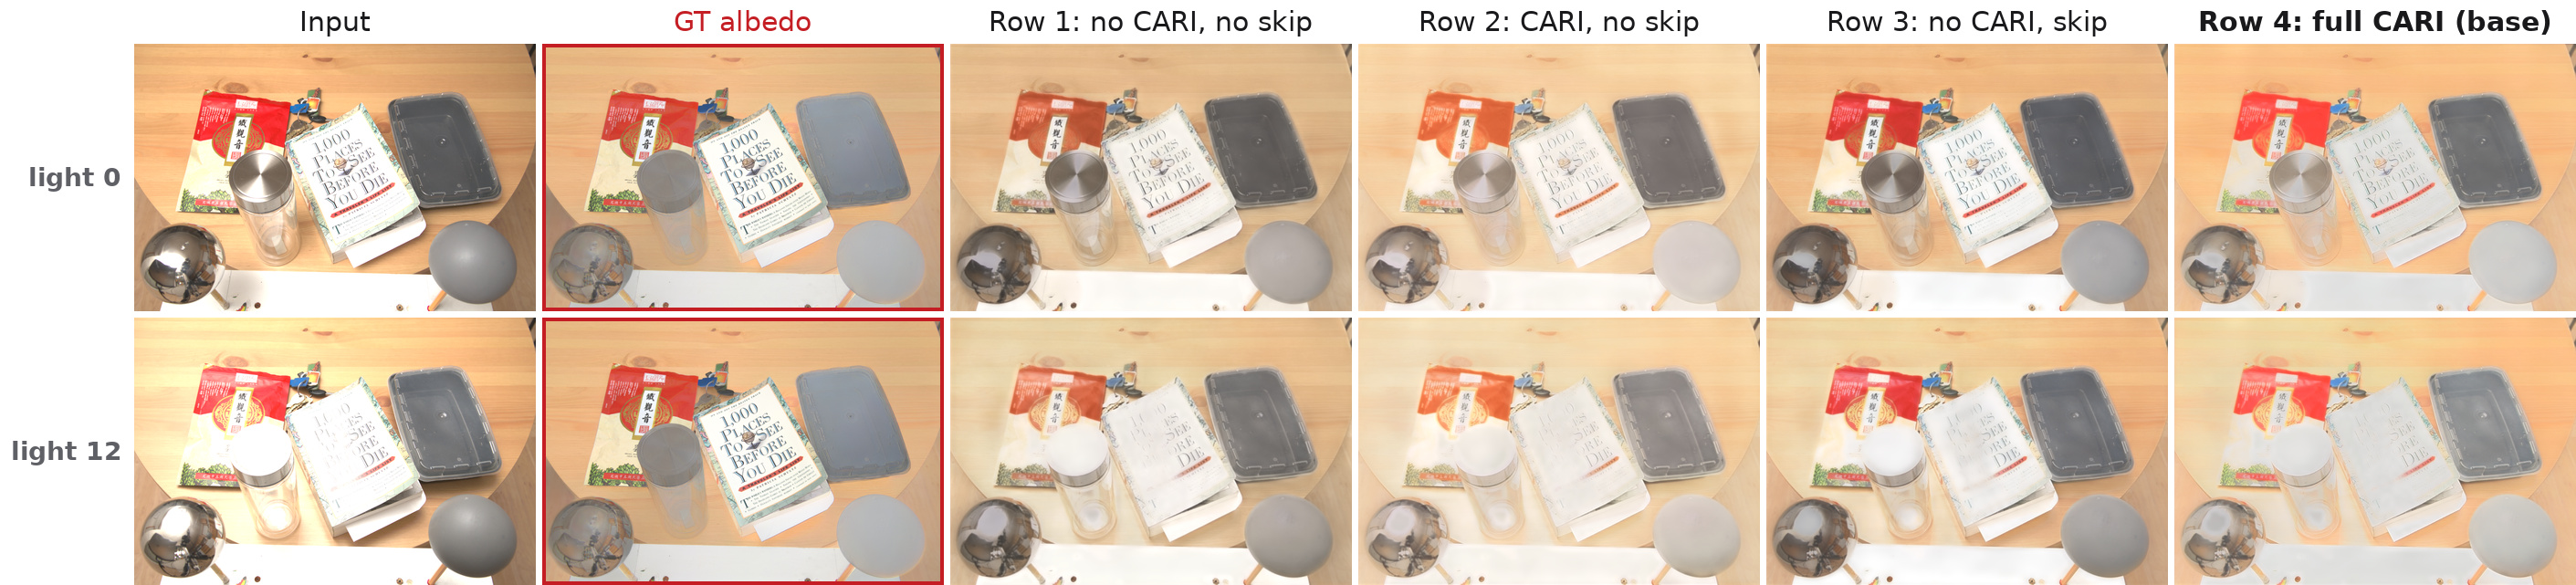
\includegraphics[width=\textwidth]{images/hires/ablation_mid.jpg}
  \caption[Qualitative CIAI ablation on MID.]{%
    The four ablation rows on one MID scene. Columns: three of the input flash directions
    (L0, L10, L20), the pseudo-ground-truth albedo (red box), the three predicted albedos,
    and two variation maps over five directions (L0, L5, L10, L15, L20): the luminance
    coefficient of variation, which matches $C_{\text{mat}}$, and a chroma variation
    $\sqrt{\mathrm{Var}(R/G) + \mathrm{Var}(B/G)}$, shown for illustration only. Rows, top to
    bottom: no CIAI (Row~1), cross-illumination only (Row~2), colour path only (Row~3), and full
    CIAI (Row~4). One scene cannot rank the rows; \tabref{tab:ablation} does.
  }
  \label{fig:ablation}
\end{figure}


\section{IIW: Perceptual Reflectance Ordering}
\label{sec:iiw_results}

\begin{figure}[t!]
  \centering
  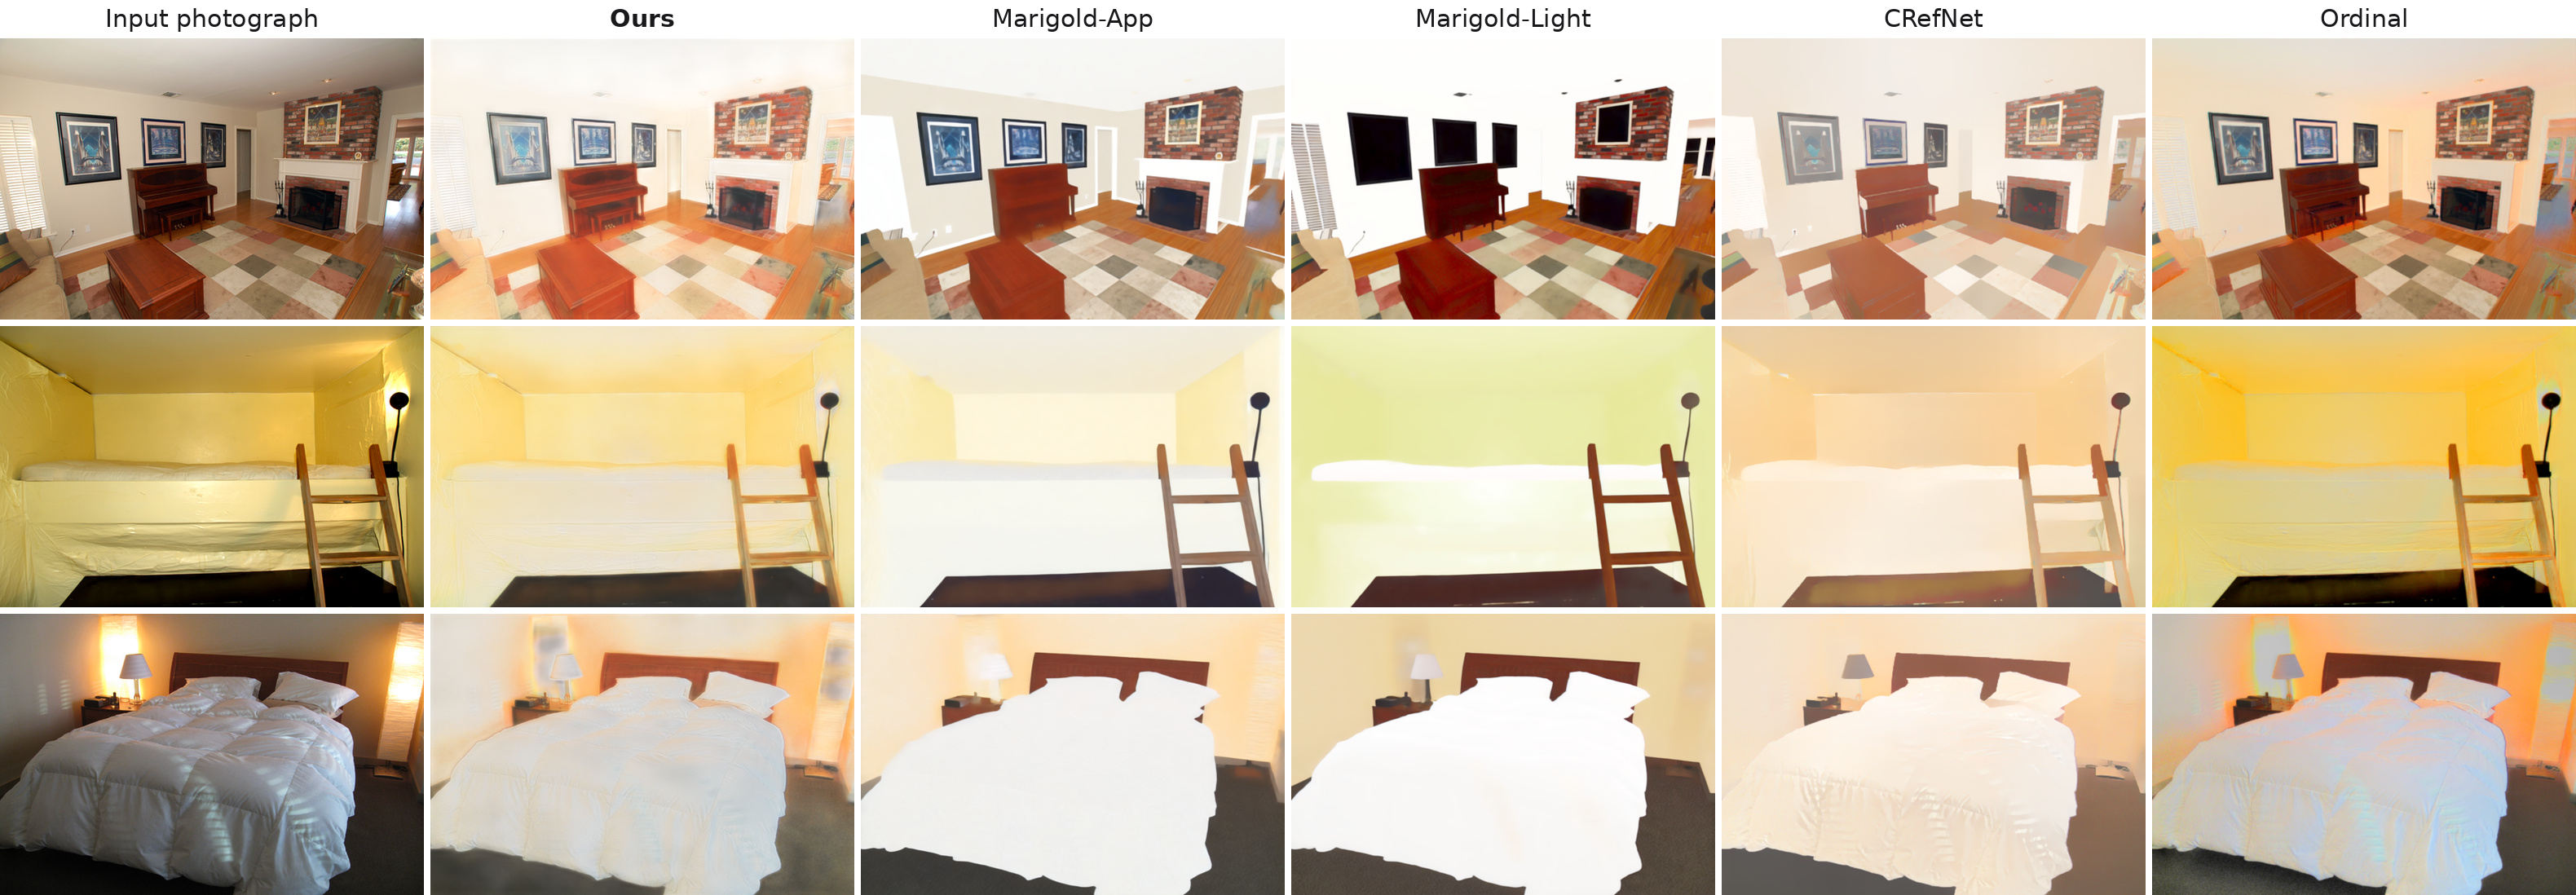
\includegraphics[width=\textwidth]{images/hires/comp_grid.jpg}
  \caption[Qualitative IIW albedo comparison across methods.]{%
    Qualitative albedo comparison on in-the-wild photographs (IIW), all methods run under
    the identical evaluation protocol. Each panel is scale-normalised by its own
    99th percentile, because albedo is defined only up to a global scale and each method
    fixes that scale differently; beyond this, no colour correction is applied.
    IIW has no albedo ground truth (\figref{fig:datasets}), so an albedo that looks cleaner
    cannot be told apart by eye from one whose colour has been removed. The diffusion
    baselines whiten these interiors more than we do; on MID, where pseudo-ground truth
    exists, Marigold-App and CRefNet have a chroma error of $0.195$ and $0.201$ against our
    $0.129$ (\tabref{tab:mid}). The figure therefore shows how each method behaves, not
    which is correct.
  }
  \label{fig:comp_grid}
\end{figure}

The purpose of this section is to check that CIAI does not damage the relative lightness of
surfaces as people judge it. IIW (\secref{sec:benchmarks}) scores a prediction with WHDR,
the confidence-weighted fraction of human lightness comparisons that the predicted albedo
orders the wrong way,
\begin{equation}
  \text{WHDR} \;=\;
  \frac{\sum_{i} w_i \cdot \mathbb{1}\bigl[\hat{r}_i \neq r_i\bigr]}{\sum_{i} w_i},
  \label{eq:whdr}
\end{equation}
where $r_i$ is the human verdict on the $i$-th pair (lighter, darker, or equal),
$\hat{r}_i$ is the verdict implied by the predicted albedo under a threshold on the
ratio of the two points' intensities, and $w_i$ is the annotator confidence.
Lower is better.

\eqnref{eq:whdr} shows two limits of the score. First, $\hat{r}_i$ depends only on the
\emph{ratio} of two predicted intensities, so WHDR ignores colour: a model can tint every
surface with the colour of the lamp and lose nothing, as long as the relative lightness of the
pairs survives. Second, the labels are sparse lightness orderings, so they cannot determine
absolute intensity, chromaticity or texture \mycite{maw,sato25metrics}. Moreover, each IIW
image is seen under one light, so WHDR cannot test stability either. We therefore read it as
a check that CIAI does not damage lightness ordering, and turn to MAW
(\secref{sec:maw_results}) for material colour.

\tabref{tab:iiw} separates the locally evaluated rows from cited results. The cited rows
are context only, because each source uses its own inference code and protocol.

\begin{table}[t!]
  \caption[IIW WHDR results.]{%
    Results on IIW \mycite{bell14iiw}. WHDR is lower-is-better. The upper block
    is evaluated locally; rows using IIW supervision are identified explicitly. The cited block
    is the no-IIW-supervision rows of Ordinal Shading \mycite{careaga23ordinal}, Table~2.
    $\dagger$ marks a result obtained with IIW supervision under a different protocol.
  }
  \label{tab:iiw}
  \centering
  \small
  \begin{tabular}{@{}lc@{}}
    \toprule
    Model & WHDR $\downarrow$ \\
    \midrule
    Ours & 0.286 \\
    Marigold-App \mycite{marigoldiid24} & 0.193 \\
    Marigold-Light \mycite{marigoldiid24} & 0.215 \\
    CRefNet (local; IIW-supervised) \mycite{luo23crefnet} & \textbf{0.168} \\
    Ordinal (local) \mycite{careaga23ordinal} & 0.257 \\
    \midrule
    \multicolumn{2}{@{}l}{\itshape\small Cited from Ordinal Shading, Table~2 (no IIW supervision):}\\
    Bell et al. \mycite{bell14iiw} & 0.206 \\
    CGIntrinsics \mycite{li18cgintrinsics} & 0.178 \\
    NIID-Net \mycite{luo20niid} & 0.166 \\
    PIE-Net \mycite{das22pienet} & 0.213 \\
    Ordinal Shading \mycite{careaga23ordinal} & 0.249 \\
    \midrule
    \multicolumn{2}{@{}l}{\itshape\small Original CRefNet result (different protocol):}\\
    CRefNet$^\dagger$ \mycite{luo23crefnet} & 0.108 \\
    \bottomrule
  \end{tabular}
\end{table}

As can be seen from \tabref{tab:iiw}, our model's WHDR of $0.286$ trails every locally
evaluated baseline, including Ordinal Shading ($0.257$). However, within the ablation of
\secref{sec:ablation}, adding CIAI improves WHDR (0.334 to 0.283 without the colour path, 0.327
to 0.286 with it). The pair losses therefore help lightness ordering rather than hurt it, and
the gap to other methods lies in the base model. \figref{fig:iiw} shows qualitative results
on the IIW test set.

\begin{figure}[t!]
  \centering
  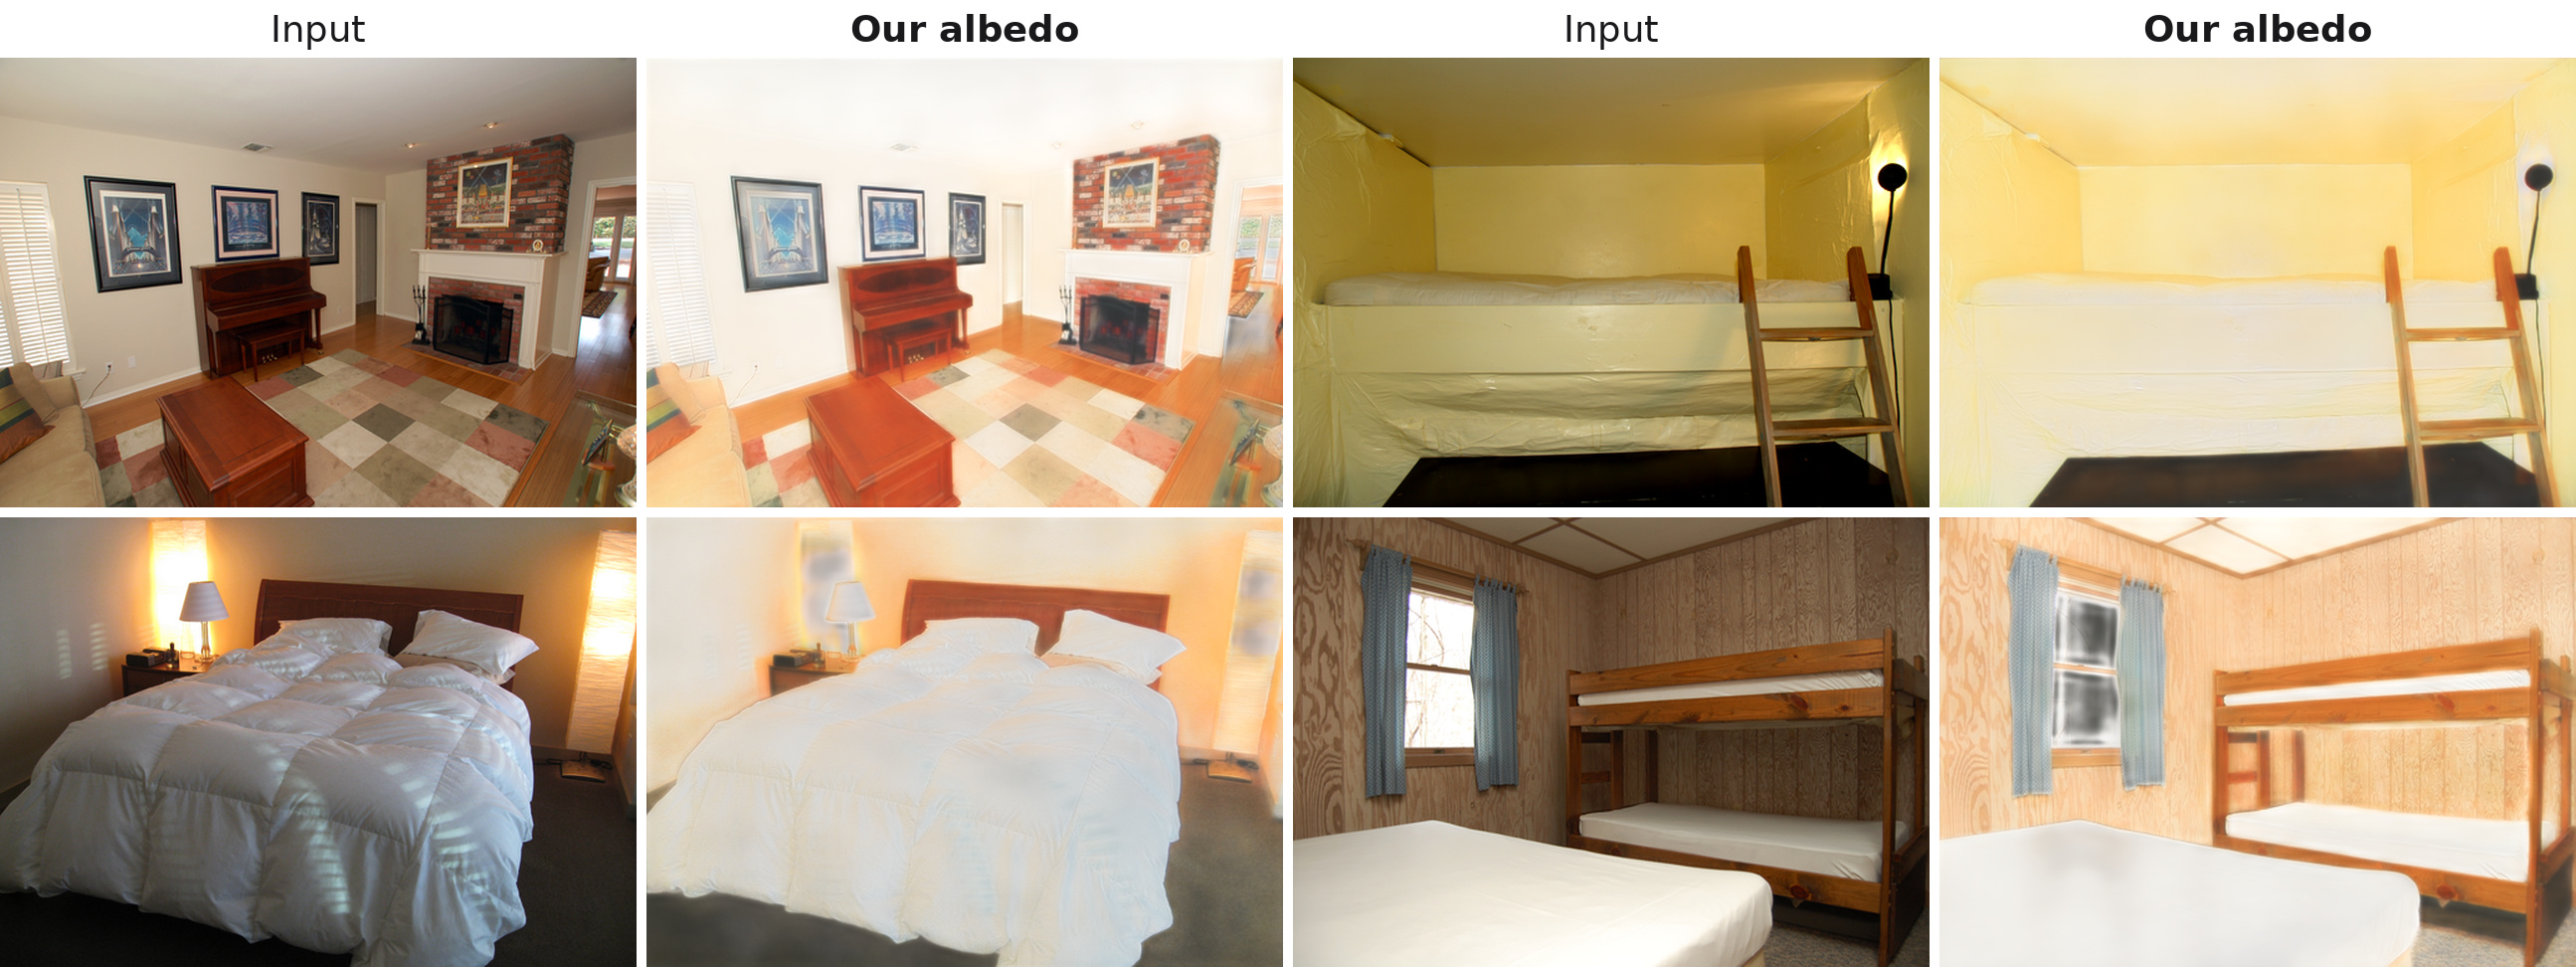
\includegraphics[width=0.85\textwidth]{images/hires/iiw_ours.jpg}
  \caption[IIW qualitative predictions and failure cases.]{%
    Qualitative albedo predictions from our model on IIW test images.
    Each row shows an input image (left) and its predicted albedo (right).
    The predictions preserve broad material regions but show the two competing
    errors that an ordinal score can expose only at annotated point pairs:
    legitimate material boundaries may be over-smoothed, while illumination
    structure remains on the ceiling and around the windows. IIW has no measured albedo, so
    the figure shows failure modes, not colour accuracy.
  }
  \label{fig:iiw}
\end{figure}


\section{MAW: Measured Real-World Albedo}
\label{sec:maw_results}

The purpose of this section is to test whether the predicted material colour is correct, not
only stable. MAW (\secref{sec:maw_dataset}) measures albedo on real surfaces, so it catches a
model that is stable across lights (a low $C_{\text{mat}}$) but consistently wrong about the
colour of the wall. Its public scorer reports two scores, both after removing scale
(\secref{sec:app_maw}). $\Delta E$ is a CIEDE2000 colour difference after aligning the
intensity of each material separately, so it is mainly a chromaticity test and our primary
external colour score. The intensity SI-MSE fits one global scale and then scores the
\emph{relative} lightness of the materials. Lower is better for both. We run every local
method with the common inference cap of \secref{sec:exp_setup}, which matches the MAW
protocol of CD-IID \mycite{careaga24cdiid}; the cited block of \tabref{tab:maw} keeps only
methods reported under that protocol, with CD-IID Table~1 as the primary reference.

\begin{table}[t!]
  \caption[MAW albedo accuracy results.]{%
    Results on MAW \mycite{maw}, evaluated with the benchmark scorer.
    $\Delta E$ measures CIELAB colour difference and intensity
    SI-MSE$\times100$ measures scale-invariant brightness error; lower is
    better for both. The upper block is evaluated locally. The complete lower
    block is transcribed from CD-IID \mycite{careaga24cdiid}, Table~1. The colour-path-only
    row is Row~3 of the ablation (no CIAI), shown for reference.
    $^{*}$ denotes the grayscale-shading assumption, for which predicted
    chromaticity is inherited from the input image. Red, orange, and yellow
    cells mark first, second, and third place over the common protocol.
  }
  \label{tab:maw}
  \centering
  \small
  \begin{tabular}{@{}lcc@{}}
    \toprule
    Model & $\Delta E$ $\downarrow$ & Int. SI-MSE$\times$100 $\downarrow$ \\
    \midrule
    Ours                                       & 4.155 & \rankthree{0.504} \\
    Ours, colour path only (ablation Row~3)    & 4.115 & \rankone{0.395} \\
    Marigold-App \mycite{marigoldiid24}        & \ranktwo{3.775} & 0.653 \\
    Marigold-Light \mycite{marigoldiid24}      & 4.214 & \ranktwo{0.493} \\
    CRefNet \mycite{luo23crefnet}              & \rankthree{3.970} & 0.942 \\
    Ordinal (local) \mycite{careaga23ordinal}  & 6.884 & 0.657 \\
    \midrule
    \multicolumn{3}{@{}l}{\itshape\small Cited from CD-IID, Table~1:}\\
    Bell et al. \mycite{bell14iiw}             & 6.61 & 3.11 \\
    CGIntrinsics \mycite{li18cgintrinsics}     & 5.15 & 2.71 \\
    Li \& Snavely$^{*}$ \mycite{li18bigtime} & 6.56 & 1.72 \\
    NIID-Net \mycite{luo20niid}                & 4.73 & 1.24 \\
    IRISformer \mycite{zhu22irisformer}        & 4.94 & 1.44 \\
    Kocsis et al. \mycite{kocsis24iid}         & 5.35 & 1.13 \\
    IntrinsicAnything \mycite{chen24intrinsicanything} & 4.12 & 0.98 \\
    Ordinal Shading$^{*}$ \mycite{careaga23ordinal} & 6.56 & 0.57 \\
    CD-IID \mycite{careaga24cdiid}             & \rankone{3.37} & 0.54 \\
    \bottomrule
  \end{tabular}
\end{table}

As can be seen from \tabref{tab:maw}, our model is mid-table on measured albedo: its colour error ($\Delta E = 4.155$) is behind
CD-IID, Marigold-App and CRefNet, and its relative-intensity error ($0.504$) is among the
lowest. CIAI itself slightly worsens both MAW measures in the ablation (4.115 to 4.155 and
0.395 to 0.504 with the colour path). The gain in stability therefore comes with a small
cost in single-image accuracy on MAW, and we report the two together.

\figref{fig:maw} shows a representative MAW scene.
The ground-truth panel is masked to the surface regions whose albedo was
physically measured by the dataset authors; only those regions enter the
score.

\begin{figure}[t!]
  \centering
  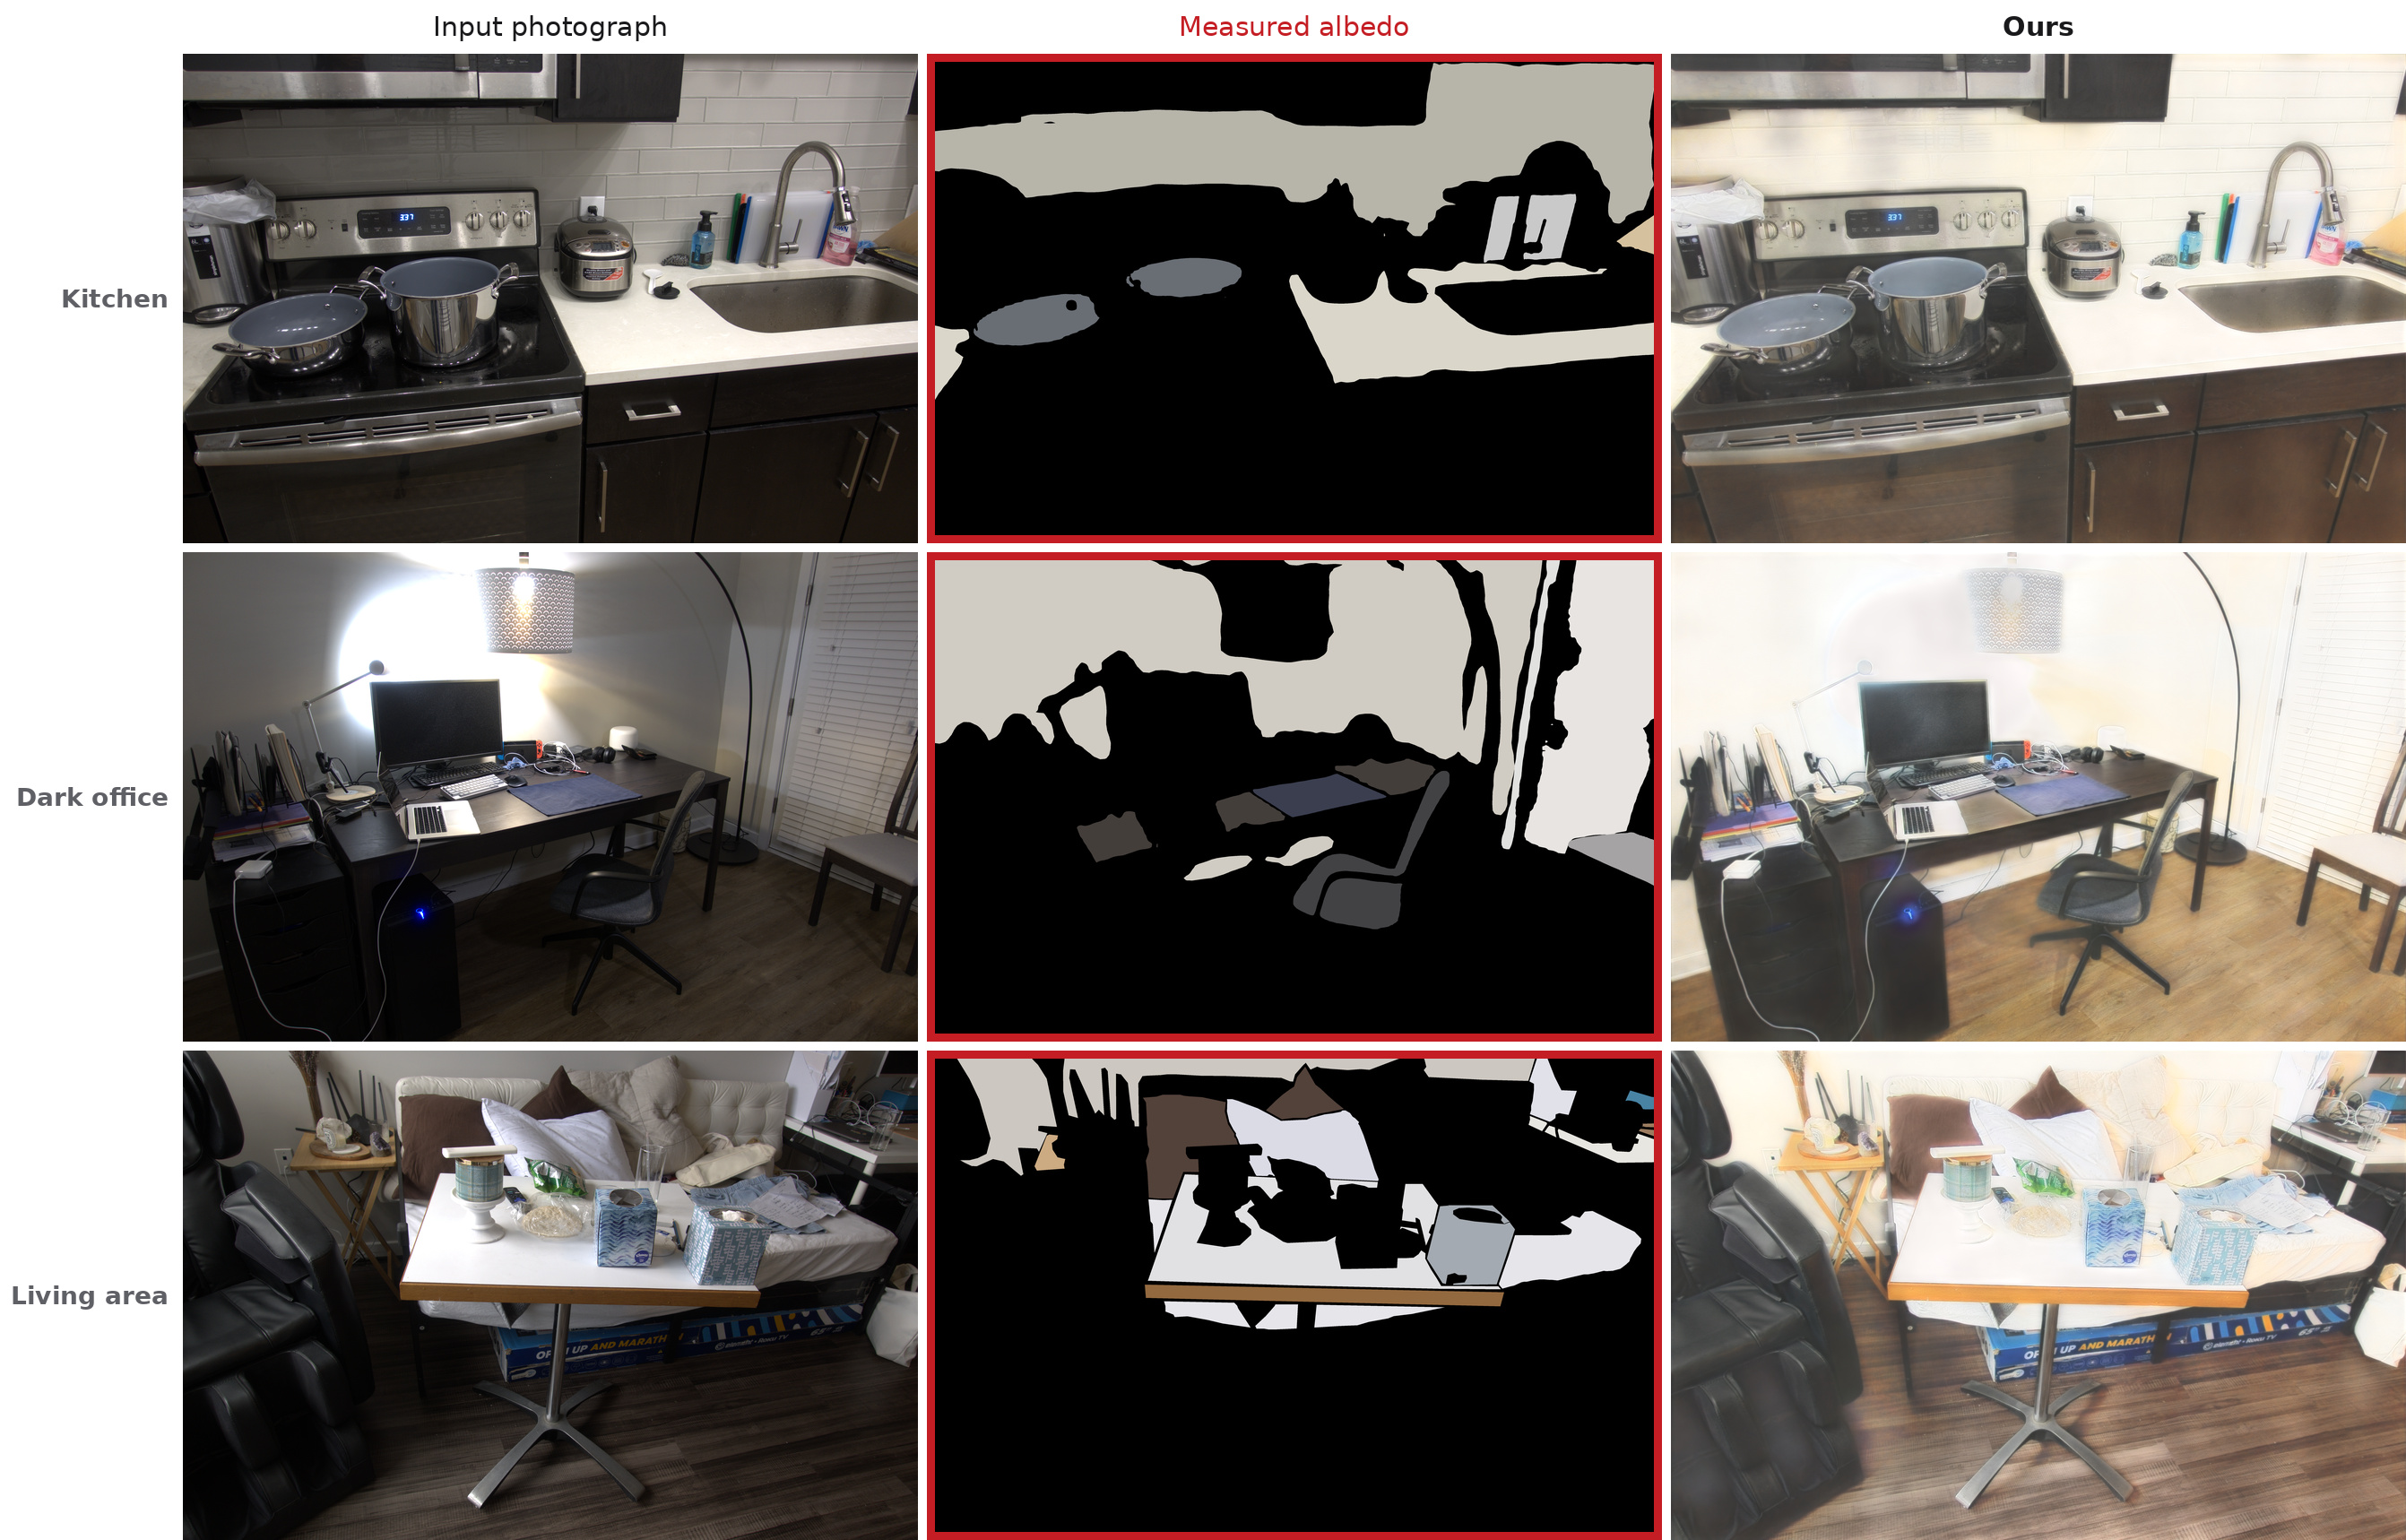
\includegraphics[width=\textwidth]{images/hires/maw_ours.jpg}
  \caption[Qualitative MAW albedo comparison.]{%
    Qualitative comparison on three content-diverse MAW photographs (one per
    row): a kitchen, a dark office, and a living area. Left to right: input
    photograph, measured albedo (red border and masked to reliable regions),
    and our prediction.
  }
  \label{fig:maw}
\end{figure}


\section{ARAP: Constancy and Albedo Accuracy}
\label{sec:arap_results}

The purpose of this section is to measure stability and accuracy on the same pixels. ARAP
\mycite{arap} is the only benchmark here with dense ground-truth albedo \emph{and} several
renderings of the same scene under different lights: MID has the repeated lights but no true
albedo, and MAW has the true albedo but one light per surface. It is synthetic, however, so a
good ARAP number cannot by itself support a claim about real rooms, and we report it last.

\paragraph{Evaluation mask}
ARAP stores its ground-truth albedo in three encodings: 40 scenes divided by the Radiance
constant $179$ (maximum about $0.0056$), seven 8-bit sRGB scenes, and four unscaled ones. We
score the pixels whose ground-truth albedo luminance exceeds a fixed $0.004$. This keeps a
median of $1.5\%$ of the frame in the first group and about $99\%$ in the others, and it
leaves six scenes empty, so $136$ of the $157$ images are scored. Every model passes through
the same mask, so the comparisons between models are consistent, but the absolute ARAP
values are not comparable with published numbers. Our mean-normalised RMSE is also not the
least-squares scale-invariant RMSE of published ARAP tables. For this reason no claim in this
thesis rests on ARAP alone.

\paragraph{Two questions}
ARAP answers two questions, which we keep apart. First, does a prediction stay stable when
the coloured illumination changes? We test this on the raw renderings
(\tabref{tab:arap_constancy}). Second, how accurate is the albedo when the input is neutrally
lit? We test this on white-balanced input against the dense ground truth
(\tabref{tab:arap_accuracy}).

For the second question, a global exposure rescale is not enough, because multiplying all
three channels by one scalar leaves the illuminant colour unchanged. We instead rebuild a
neutrally lit image from the ground-truth albedo: with the implied shading
$\mathbf{S}=\mathbf{I}/\mathbf{A}^{*}$, we recompose
$\mathbf{I}_{\text{wb}} = \mathbf{A}^{*}\cdot\mathrm{lum}(\mathbf{S})$, whose implied
illuminant is exactly neutral. The stability table keeps the raw renderings, because removing
the illuminant would remove the variable under test.

The stability table uses only the groups whose illuminant \emph{colour} changes between
renderings ($16$ groups, $11$ indoor). Groups that vary only intensity or direction would pull
every model's score toward zero. The accuracy table scores all 136 usable images and adds
published original-ARAP results from Ordinal Shading \mycite{careaga23ordinal}, Table~1.

\begin{table}[t!]
  \caption[ARAP cross-illumination constancy.]{%
    ARAP stability on raw inputs, over the $16$ groups ($11$ indoor) of \mycite{arap} whose
    illuminant colour changes between renderings. $C_{\text{arap}}$ (\eqnref{eq:carap}) is the
    per-pixel variation of predicted albedo luminance across a group; lower is better. Red, orange, and yellow mark first, second, and third numerical rank in
    each column; displayed ties share a rank. These are internal diagnostics, evaluated
    locally.
  }
  \label{tab:arap_constancy}
  \centering
  \begin{tabular}{@{}lcc@{}}
    \toprule
    & All & Indoor \\
    & ($n{=}16$) & ($n{=}11$) \\
    \cmidrule(lr){2-2}\cmidrule(l){3-3}
    Model & $C_{\text{arap}}$ $\downarrow$ & $C_{\text{arap}}$ $\downarrow$ \\
    \midrule
    Ours                                       & \rankthree{0.154} & \ranktwo{0.119} \\
    Marigold-App \mycite{marigoldiid24}        & \rankone{0.113} & \rankone{0.113} \\
    Marigold-Light \mycite{marigoldiid24}      & 0.340 & 0.340 \\
    CRefNet \mycite{luo23crefnet}              & \ranktwo{0.128} & \rankthree{0.129} \\
    Ordinal Shading \mycite{careaga23ordinal}  & 0.175 & 0.165 \\
    \bottomrule
  \end{tabular}
\end{table}

\begin{table}[t!]
  \caption[ARAP dense-albedo accuracy.]{%
    ARAP albedo accuracy, \emph{within-study}, on the full Bonneel et al. collection
    \mycite{arap} (136 of 157 images have dense ground-truth albedo with enough valid
    pixels to score; the same 136 are used for every model). Input is white-balanced by
    reconstructing an achromatic-illuminant image from the ground-truth albedo
    (\secref{sec:arap_results}). LMSE and mean-normalised RMSE are lower-is-better, SSIM
    higher. The upper block is evaluated locally under one harness; the lower
    block is transcribed from Ordinal Shading \mycite{careaga23ordinal},
    Table~1, and reports no SSIM because that protocol is unspecified (see the
    note below the table). Red, orange, and yellow mark first, second, and third
    place; LMSE and mn-RMSE rank across all rows, SSIM within the local block.
  }
  \label{tab:arap_accuracy}
  \centering
  \small
  \begin{tabular}{@{}lccc@{}}
    \toprule
    Model & LMSE $\downarrow$ & mn-RMSE $\downarrow$ & SSIM $\uparrow$ \\
    \midrule
    Ours                                       & 0.0279 & \ranktwo{0.2259} & \ranktwo{0.611} \\
    Marigold-App \mycite{marigoldiid24}        & 0.0266 & 0.2529 & \rankthree{0.607} \\
    Marigold-Light \mycite{marigoldiid24}      & 0.0706 & 0.6187 & 0.589 \\
    CRefNet \mycite{luo23crefnet}              & 0.0223 & 0.2916 & \rankone{0.622} \\
    \midrule
    \multicolumn{4}{@{}l}{\itshape\small Published original-ARAP protocol (Ordinal Shading, Table~1):}\\
    Chromaticity \mycite{arap}                 & 0.024 & 0.296 & --- \\
    NIID-Net \mycite{luo20niid}                & \rankthree{0.022} & \rankone{0.206} & --- \\
    Li \& Snavely \mycite{li18bigtime}         & \rankone{0.018} & \rankthree{0.227} & --- \\
    Bell et al.\ \mycite{bell14iiw}            & 0.028 & 0.317 & --- \\
    PIE-Net \mycite{das22pienet}               & 0.026 & 0.273 & --- \\
    Ordinal Shading \mycite{careaga23ordinal}  & \ranktwo{0.021} & 0.252 & --- \\
    \bottomrule
  \end{tabular}

  \vspace{0.6em}
  {\footnotesize\raggedright
  Published SSIM values are not transcribed, because Ordinal Shading does not state how its
  SSIM is aligned, and running Ordinal Shading through our closest reconstruction gives
  $0.671$ against the $0.761$ it reports.\par}
\end{table}

The first thing we can see from \tabref{tab:arap_constancy} is that our model is not the most
stable on ARAP: Marigold-App ($0.113$) and CRefNet ($0.128$) drift less than our $0.154$ over all
groups, and on the indoor groups our $0.119$ is second. On white-balanced accuracy
(\tabref{tab:arap_accuracy}), our model has the lowest mean-normalised RMSE of the local block
($0.2259$) and the second-best SSIM, while its LMSE ($0.0279$) trails CRefNet and Marigold-App.
On ARAP, therefore, our model is competitive but does not lead. The clearer ARAP result is the
matched one: inside our architecture, CIAI lowers the raw-input albedo error by $7$--$14\%$
(\secref{sec:ablation}).

\figref{fig:arap_models} compares the models on one scene under two illuminants, and
\figref{fig:arap_constancy} shows three further interiors.

\begin{figure}[p!]
  \centering
  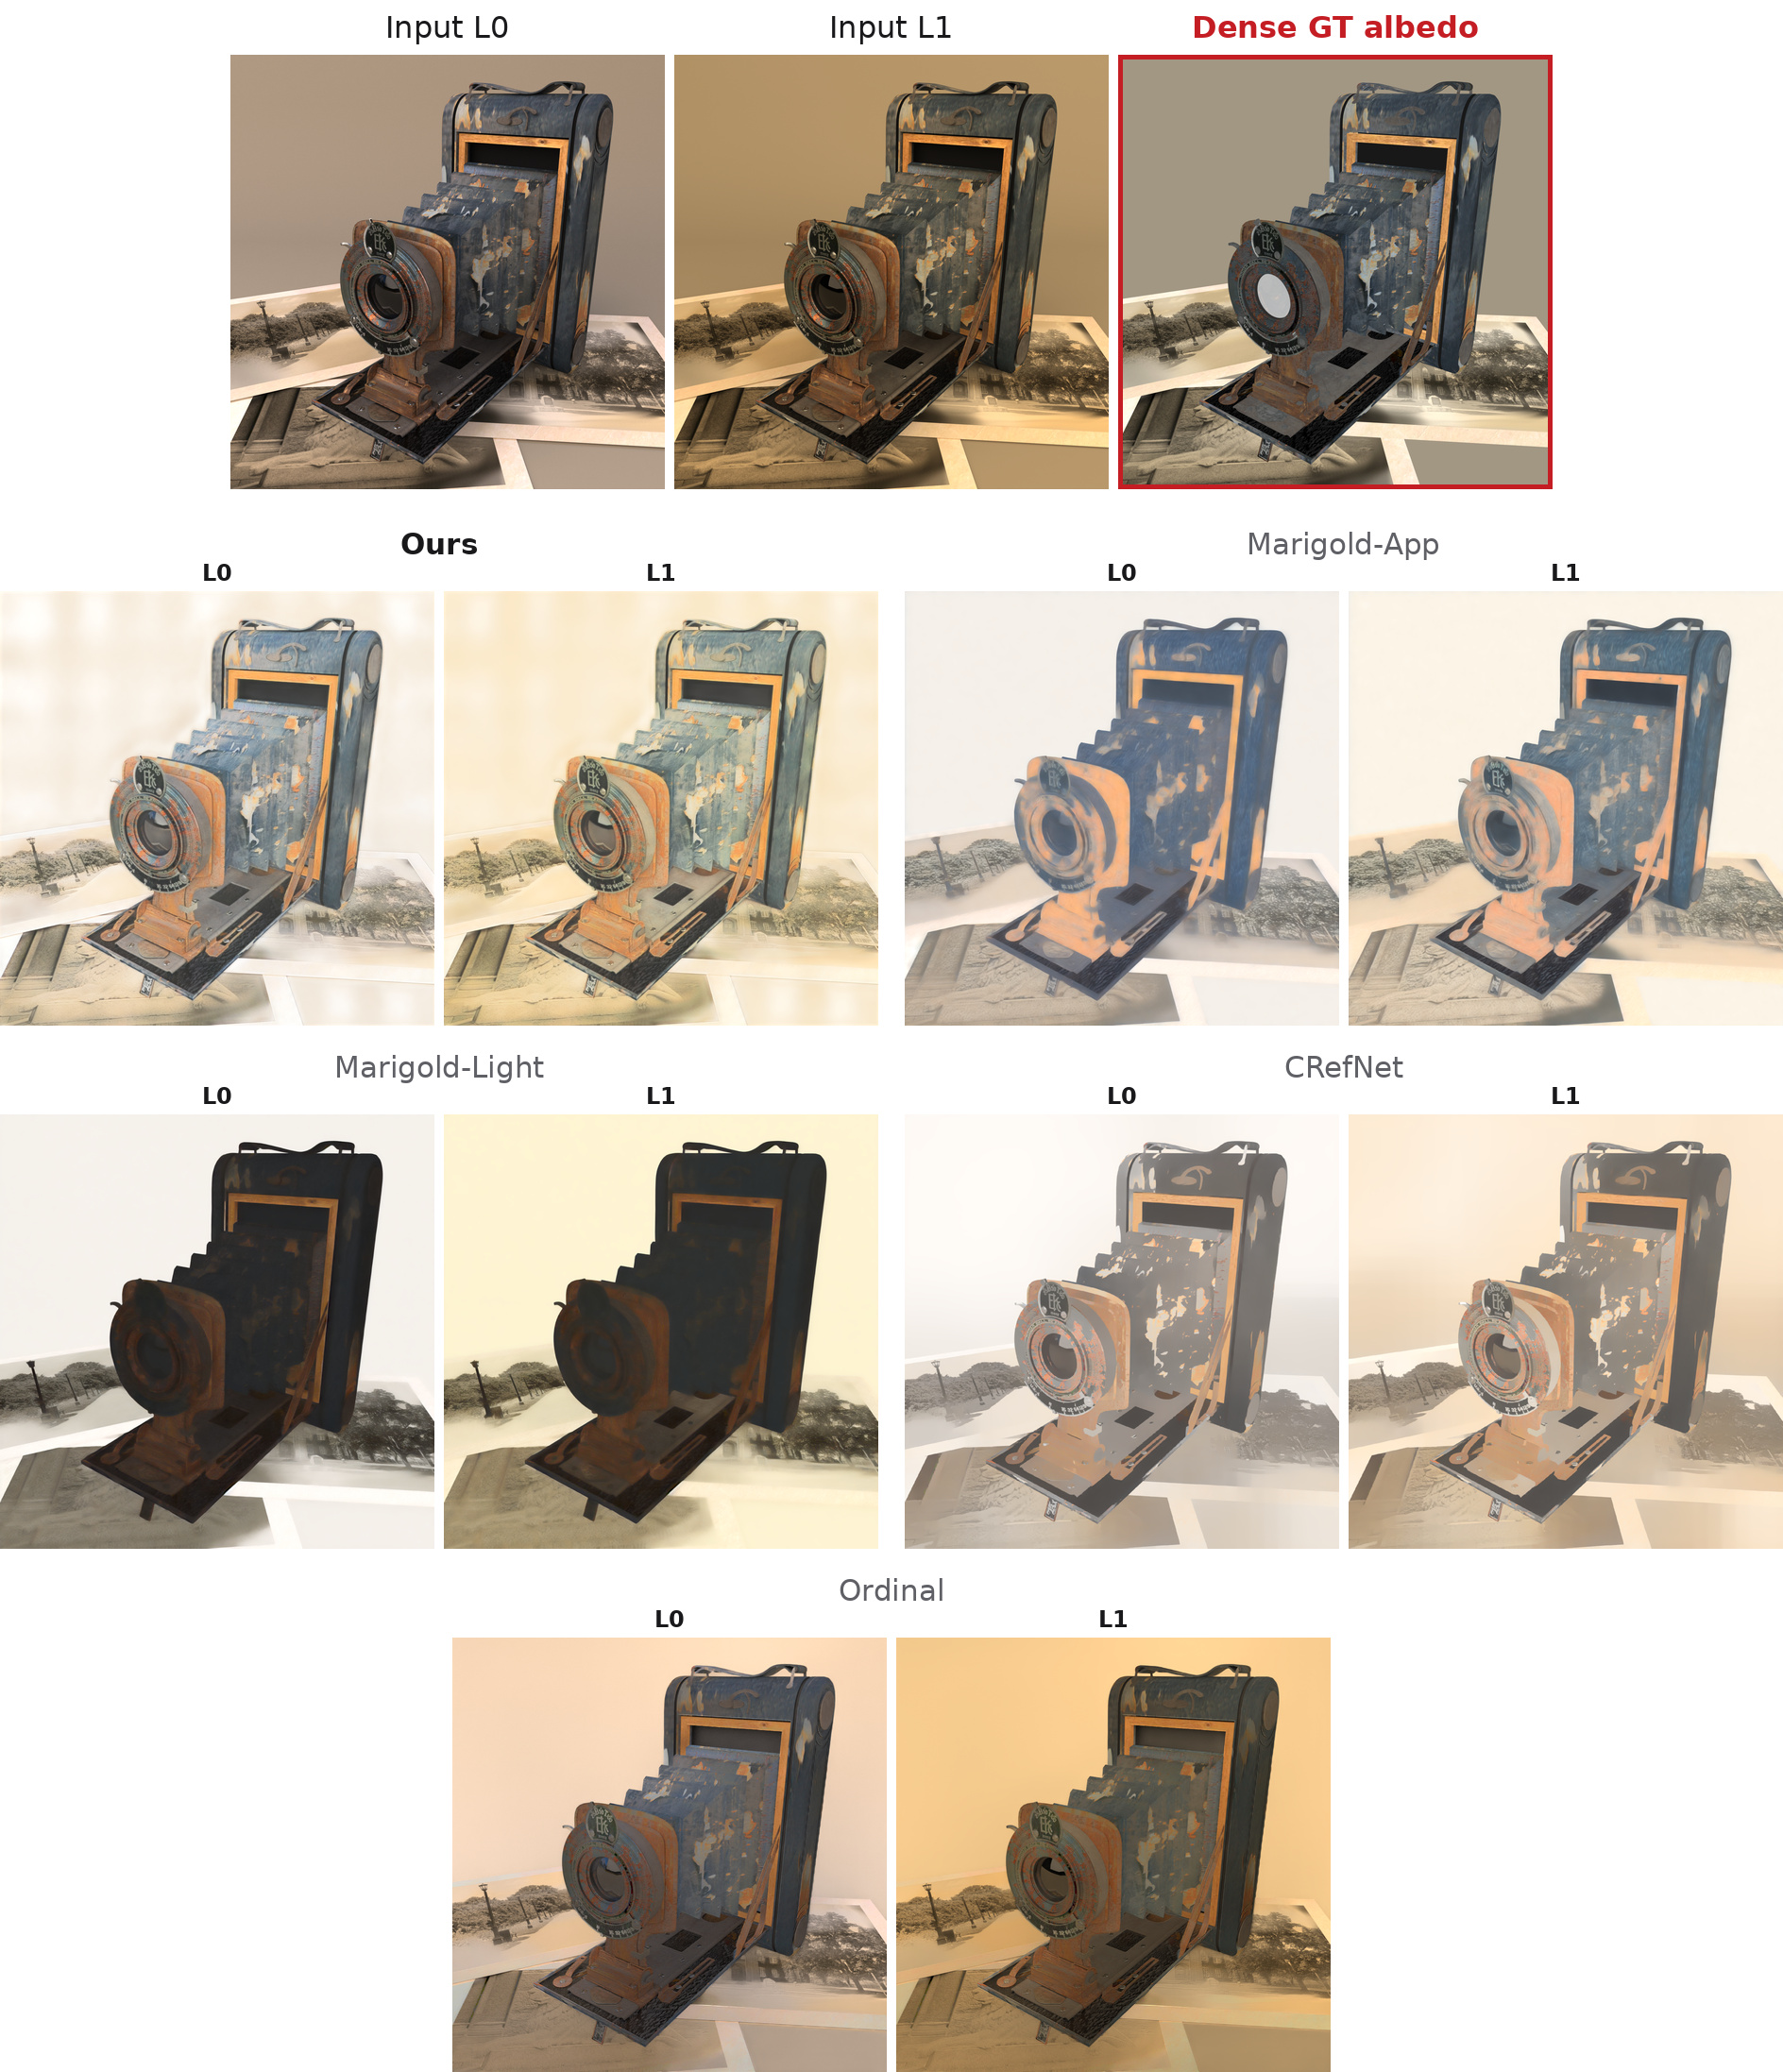
\includegraphics[width=0.98\textwidth]{images/hires/arap_model_grid.jpg}
  \caption[ARAP model comparison across illuminants on \emph{camera}.]{%
    Model-by-illuminant comparison on the ARAP \emph{camera} scene. The reference
    strip shows both rendered illuminant conditions and the dense ground-truth
    albedo once. The grid below shows each locally evaluated model's albedo under
    the same two illuminants. Predictions are scale-normalised separately for display,
    with no colour correction. Each model fails differently: CRefNet removes much of the
    material colour, Marigold-Light and Ordinal keep illumination structure, and our output
    still shows hard-shadow leakage. Marigold-App is comparatively stable on this scene.
  }
  \label{fig:arap_models}
\end{figure}

\begin{figure}[t!]
  \centering
  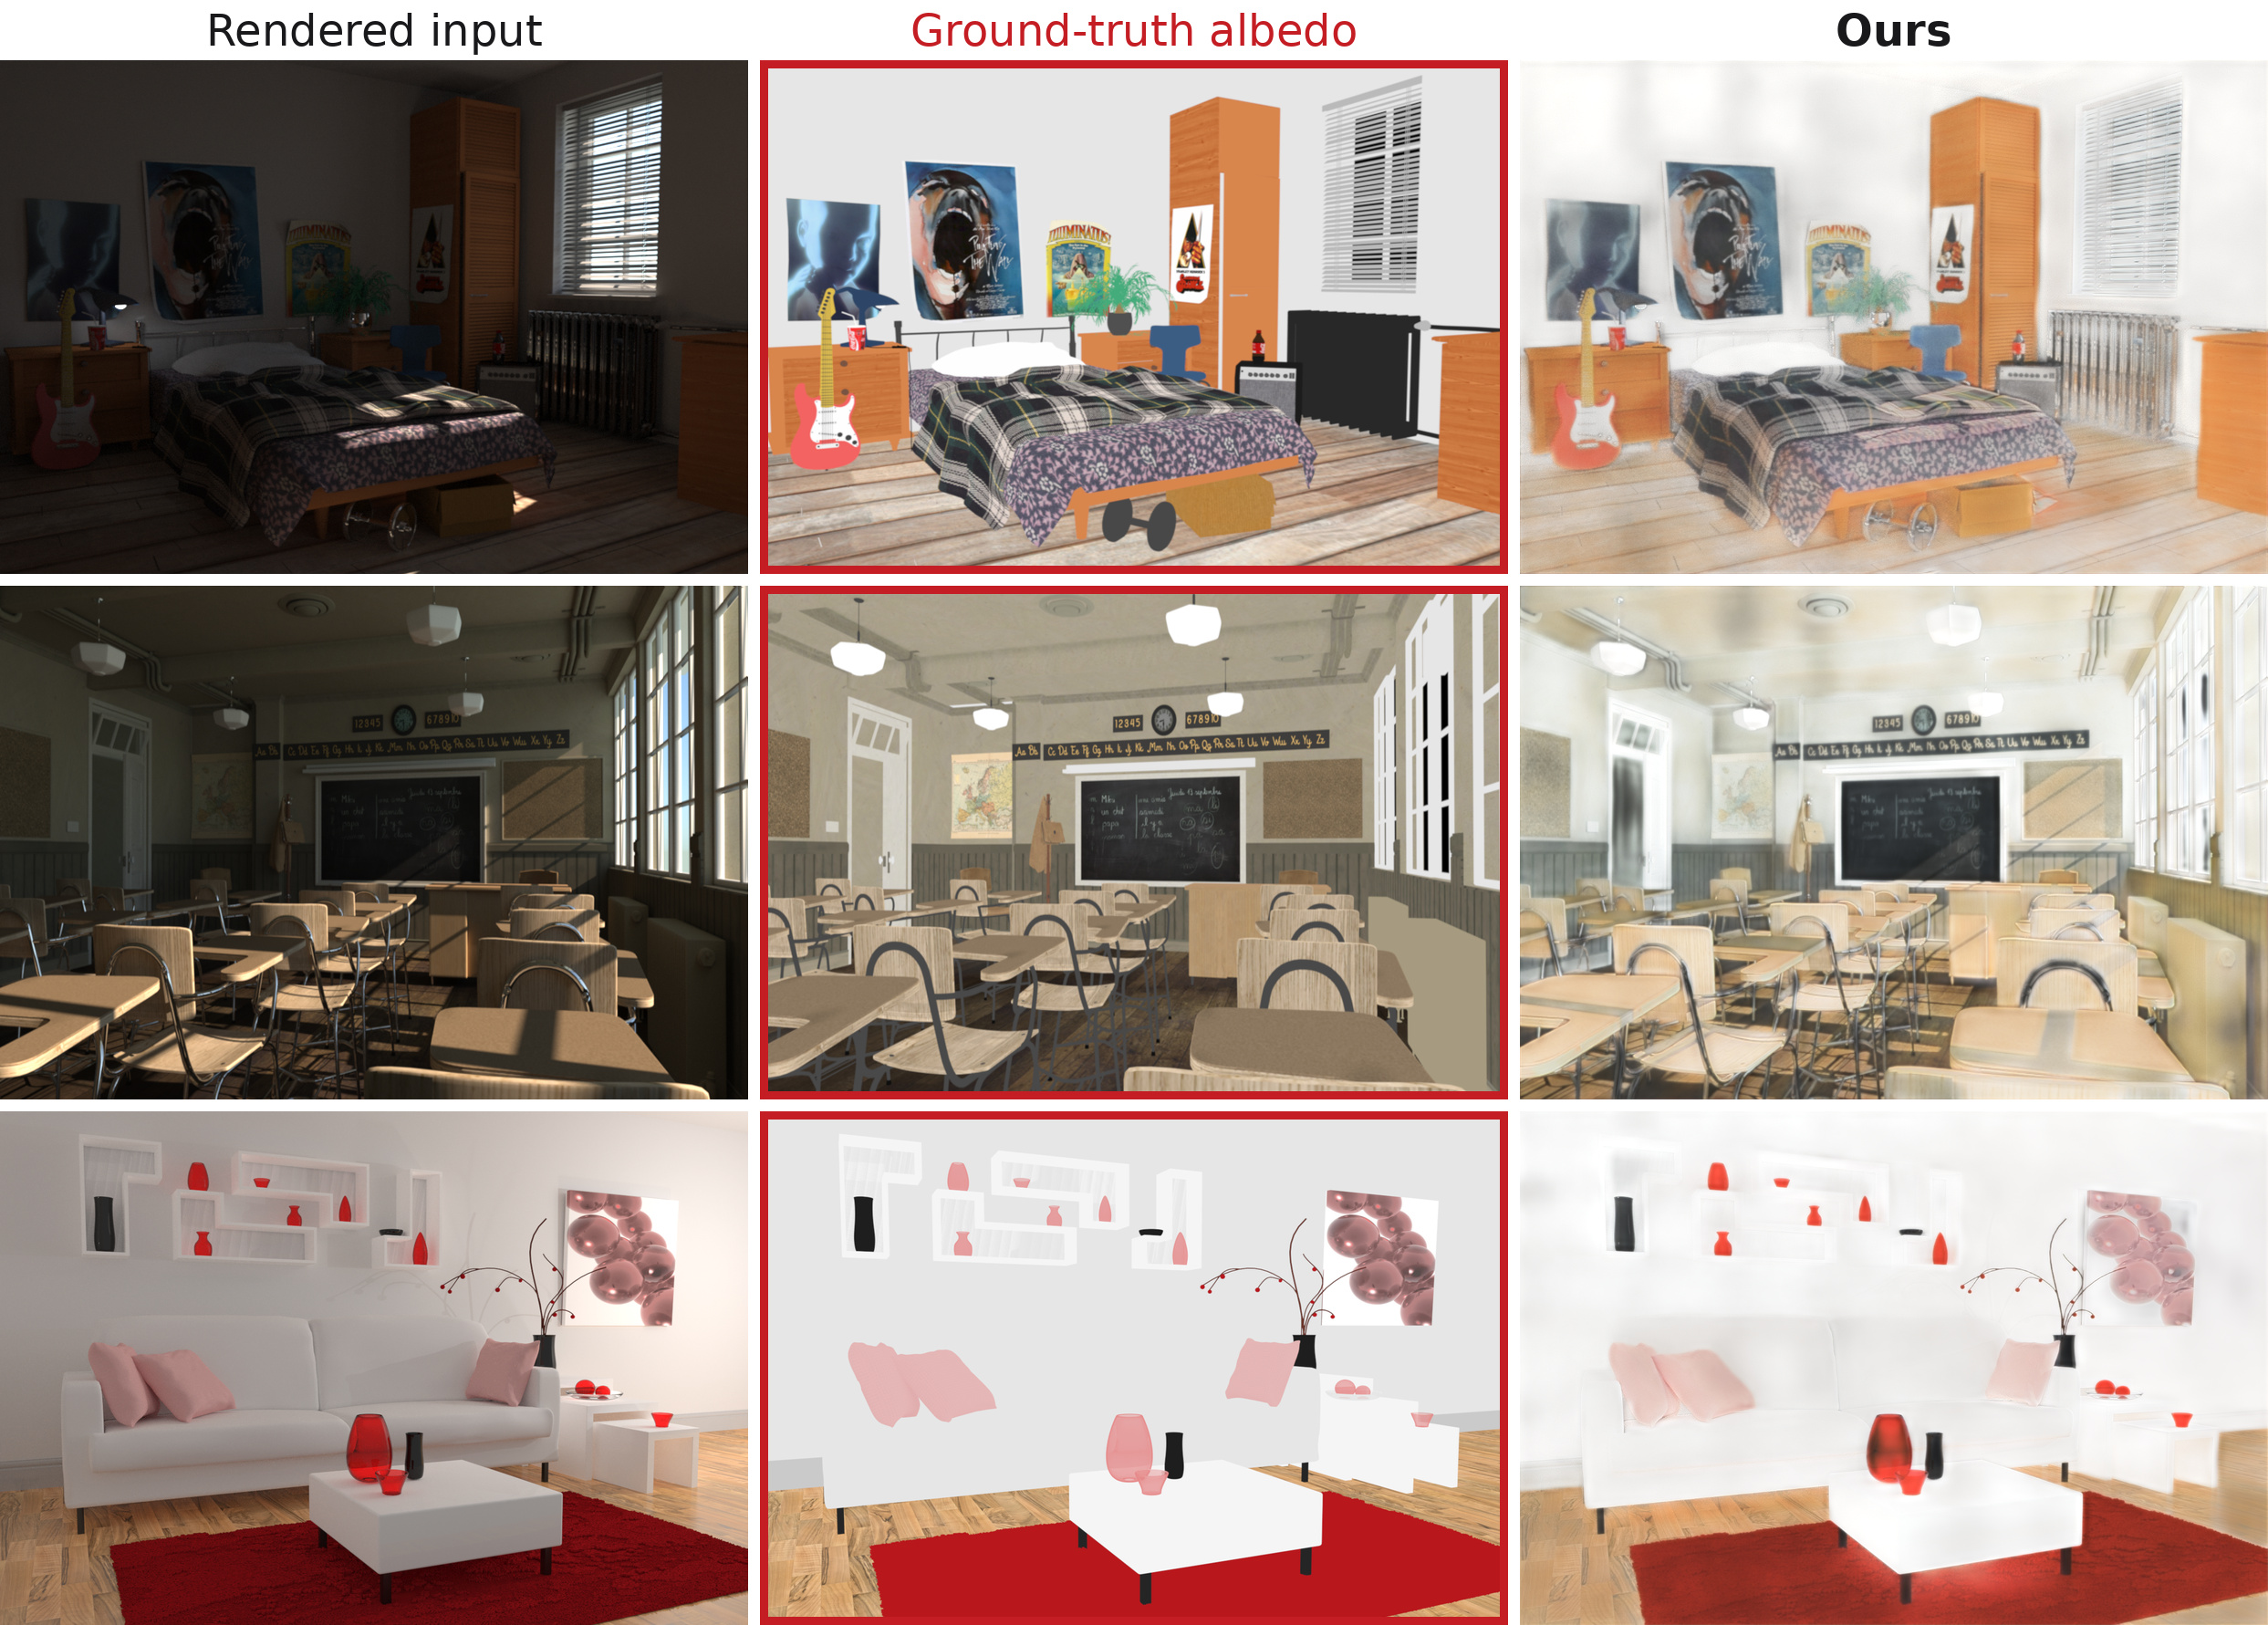
\includegraphics[width=\textwidth]{images/hires/arap_ours.jpg}
  \caption[ARAP qualitative accuracy on three indoor scenes.]{%
    Qualitative accuracy on three content-diverse ARAP scenes: \emph{bedroom},
    \emph{classroom}, and \emph{livingroom}. Each row shows the rendered input,
    dense ground-truth albedo (red border), and our prediction.
  }
  \label{fig:arap_constancy}
\end{figure}


\clearpage
\section{Colour Stability: A Limitation}
\label{sec:colour_axis}

The results so far share a pattern: CIAI improves luminance stability substantially and hue
stability barely. This is expected for two reasons. First, $\mathcal{L}_{\text{expl}}$ uses
luminance only (\secref{sec:ciai}), so nothing in CIAI states where a change in illuminant
colour must go. Second, MID's illumination changes little in colour. This section measures
the second point and checks whether our hue drift follows the illuminant colour.

\subsection{How much colour does MID's illumination vary?}

We measure the illuminant of each frame on its grey probe and take the distance between
the chromaticities $(R/\Sigma, B/\Sigma)$ of two frames of a scene as the \emph{pair gap}.
We use all 25 flash directions, the same frames on which the stability scores are computed.
For ARAP we read the illuminant from $\mathbf{I}/\mathbf{A}^*$ instead.
\figref{fig:pair_gaps} compares the two.

\begin{figure}[t!]
  \centering
  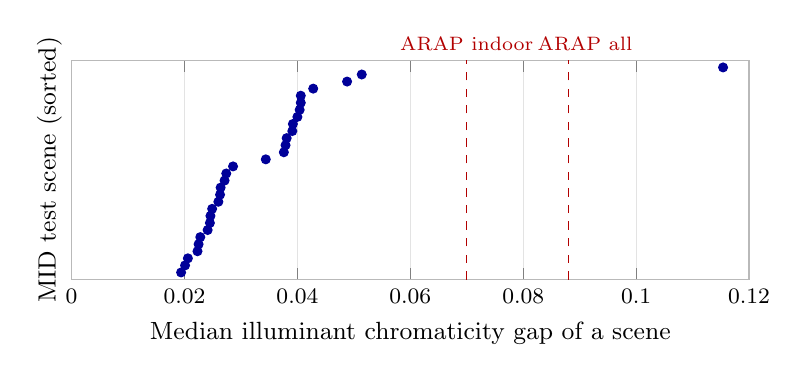
\begin{tikzpicture}
    \begin{axis}[
        width=0.84\textwidth, height=0.36\textwidth,
        xlabel={Median illuminant chromaticity gap of a scene}, ylabel={MID test scene (sorted)},
        xlabel style={font=\small}, ylabel style={font=\small}, tick label style={font=\footnotesize},
        xmin=0, xmax=0.12, ymin=0, ymax=31, ytick=\empty,
        xticklabel style={/pgf/number format/fixed, /pgf/number format/precision=2},
        scaled x ticks=false,
        grid=major, grid style={gray!22}, axis line style={gray!55}, clip=false]
      \addplot[only marks, mark=*, mark size=1.6pt, blue!60!black] coordinates {(0.0194,1) (0.0201,2) (0.0206,3) (0.0223,4) (0.0225,5) (0.0228,6) (0.0241,7) (0.0245,8) (0.0246,9) (0.0249,10) (0.0260,11) (0.0263,12) (0.0264,13) (0.0271,14) (0.0274,15) (0.0286,16) (0.0344,17) (0.0376,18) (0.0379,19) (0.0381,20) (0.0391,21) (0.0392,22) (0.0400,23) (0.0404,24) (0.0406,25) (0.0406,26) (0.0428,27) (0.0488,28) (0.0514,29) (0.1154,30)};
      \draw[dashed, red!70!black] (axis cs:0.070,0) -- (axis cs:0.070,31)
        node[above, font=\scriptsize, red!70!black] {ARAP indoor};
      \draw[dashed, red!70!black] (axis cs:0.088,0) -- (axis cs:0.088,31)
        node[above, font=\scriptsize, red!70!black, xshift=6pt] {ARAP all};
    \end{axis}
  \end{tikzpicture}
  \caption[Illuminant colour change in MID and ARAP.]{%
    How much the illuminant colour changes between two frames of one scene. Each dot is
    the median gap of one MID test scene; the dashed lines are the median gaps of ARAP
    (0.070 indoor, 0.088 for all measurable pairs). Over all frame pairs, the MID median is
    0.030, about a third of ARAP's.
  }
  \label{fig:pair_gaps}
\end{figure}

$86\%$ of MID pairs fall below $0.08$, and 29 of the 30 per-scene medians lie between
$0.019$ and $0.051$; only one scene reaches $0.115$.
MID's flash is white; what colour change there is comes from light bounced off coloured
surfaces. MID therefore teaches luminance well and colour weakly, and the hue stability
measured on it is measured over a narrow range.

\subsection{Does our hue drift follow the illuminant colour?}

If a model's hue drift is caused by the illuminant colour, it should be larger on scenes
whose illuminant colour changes more. We split the 30 test scenes into terciles by their
median pair gap and divide the mean $\text{Cast}_{\text{rel}}$ of the top tercile by that of
the bottom one; a ratio of $1$ means the drift does not follow illuminant colour.

\begin{figure}[t!]
  \centering
  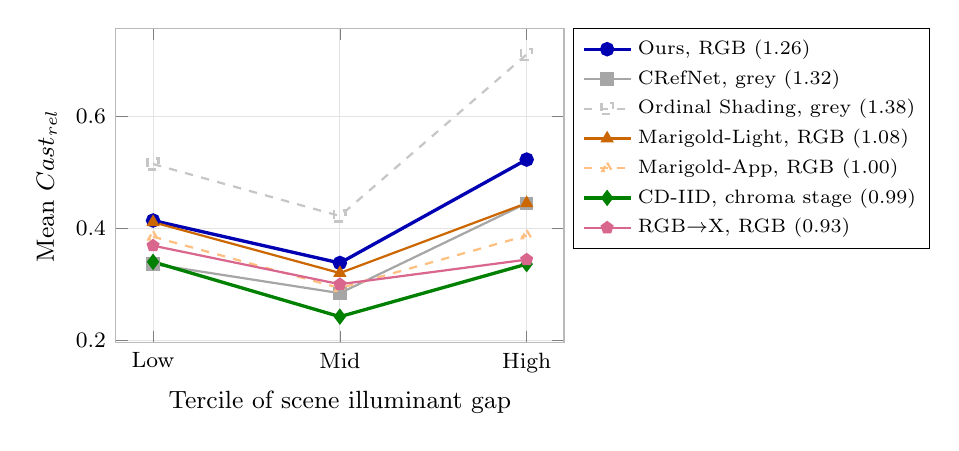
\begin{tikzpicture}
    \begin{axis}[
        width=0.6\textwidth, height=0.46\textwidth,
        xlabel={Tercile of scene illuminant gap}, ylabel={Mean $\text{Cast}_{\text{rel}}$},
        xlabel style={font=\small}, ylabel style={font=\small}, tick label style={font=\footnotesize},
        xtick={1,2,3}, xticklabels={Low, Mid, High}, xmin=0.8, xmax=3.2,
        grid=major, grid style={gray!22}, axis line style={gray!55},
        legend style={font=\scriptsize, at={(1.02,1)}, anchor=north west}, legend cell align=left]
      \addplot[very thick, blue!70!black, mark=*] coordinates {(1,0.414) (2,0.338) (3,0.523)};
      \addplot[thick, gray!70, mark=square*] coordinates {(1,0.336) (2,0.284) (3,0.445)};
      \addplot[thick, gray!45, dashed, mark=square] coordinates {(1,0.515) (2,0.422) (3,0.711)};
      \addplot[thick, orange!80!black, mark=triangle*] coordinates {(1,0.411) (2,0.320) (3,0.445)};
      \addplot[thick, orange!50, dashed, mark=triangle] coordinates {(1,0.385) (2,0.293) (3,0.387)};
      \addplot[very thick, green!50!black, mark=diamond*] coordinates {(1,0.340) (2,0.242) (3,0.336)};
      \addplot[thick, purple!60, mark=pentagon*] coordinates {(1,0.369) (2,0.300) (3,0.344)};
      \legend{{Ours, RGB (1.26)}, {CRefNet, grey (1.32)}, {Ordinal Shading, grey (1.38)},
              {Marigold-Light, RGB (1.08)}, {Marigold-App, RGB (1.00)}, {CD-IID, chroma stage (0.99)},
              {RGB$\rightarrow$X, RGB (0.93)}}
    \end{axis}
  \end{tikzpicture}
  \caption[Does hue drift follow illuminant colour?]{%
    Mean $\text{Cast}_{\text{rel}}$ per tercile of scene illuminant gap on the MID test split; the
    legend gives each method's shading type and the ratio of the high to the low tercile.
    Re-aggregated from the per-scene results behind \tabref{tab:mid}; no new inference.
  }
  \label{fig:colour_strat}
\end{figure}

\figref{fig:colour_strat} shows that our model's hue drift rises by $26\%$ on the scenes where
the illuminant colour moves most. This is close to the $32\%$ of CRefNet, whose grey
shading cannot represent a coloured light at all. In other words, CIAI's small hue gain in the ablation
(\secref{sec:ablation}) has not removed this dependence. CD-IID, the one method with a
dedicated shading-chroma stage, shows no dependence on illuminant colour ($0.99$) while keeping
its albedo colour. MID's narrow colour range makes this a low-powered test, but it agrees with
the ablation. Colour stability therefore needs a model that predicts the shading colour
separately, which is the plan of \chapref{ch:conclusion}.
